\documentclass[pdftex,12pt,a4paper]{report}

\usepackage[portuguese,english]{babel}
\usepackage[T1]{fontenc} 
\usepackage[utf8]{inputenc}
\usepackage[pdftex]{graphicx}
\usepackage{minitoc}
\usepackage{hyperref}
\usepackage{indentfirst}
\usepackage[compact]{titlesec}
\usepackage{fancyhdr}
\usepackage{caption}
\usepackage{pgfplots}
\usepackage{pgfplotstable}
\usepackage{fixltx2e}
\usepackage{mathtools}
\usepackage{fancyhdr}
\usepackage{listings}
\usepackage{color}
\usepackage{sverb}
\usepackage[section]{placeins}

%Highlight
\newcommand{\shellcmd}[1]{\indent\indent\texttt{\footnotesize\# #1}\\}

\pagestyle{fancy}
\renewcommand*\thesection{\thechapter\arabic{section}}
\newcommand{\HRule}{\rule{\linewidth}{0.5mm}}
\begin{document}

\begin{titlepage}

\begin{center}


\includegraphics[width=0.15\textwidth]{./logo}\\[0.5cm]    

\textsc{\large Universidade de Aveiro \\[1cm]\large departamento de electrónica, telecomunicações e informática}\\[1cm]

\textsc{\large{47053}\large - Computação Visual \\[1cm]}

\HRule \\[0.5cm]
{ \huge \bfseries  Puzzle}\\[0.4cm]
{ \large \bfseries Implementação em WebGL de um Puzzle}\\[0.4cm]
\HRule \\[1cm]

\textsc{\small{8240 - MESTRADO INTEGRADO EM ENGENHARIA DE COMPUTADORES E TELEMÁTICA}}\\[1cm]

\begin{minipage}{0.4\textwidth}

\begin{flushleft} \large
\href{mailto:rafael.ferreira@ua.pt}{António Rafael da \\ Costa Ferreira }
 \small{\\NMec: 67405}
\end{flushleft}
\end{minipage}
\begin{minipage}{0.4\textwidth}

\begin{flushright} \large
\href{mailto:rodrigocunha@ua.pt}{Rodrigo Lopes \\ da Cunha}
\small{\\NMec: 67800}
\end{flushright}
\end{minipage}\\[1cm]

{\large Docente: Joaquim João Estrela Ribeiro Silvestre Madeira  }\\[0.5cm]

\vfill

{\large Dezembro de 2015 \\ 2015-2016}

\end{center}

\end{titlepage} %Titulo do Relatorio
\renewcommand{\headrulewidth}{0pt}

%Cabeçalhos de rodapé
\fancyhead{}
\fancyfoot{}
\lhead{Imagens RGB - Histogramas}
\rhead{CV - 2015/2016}
\lfoot{Rafael Ferreira nmec: 67405 \\ Rodrigo Cunha nmec: 67800}
\rfoot{\thepage}

%Renomear Comandos
\renewcommand*\contentsname{Conteúdos}
\renewcommand*\figurename{Figura}
\renewcommand*\tablename{Tabela}

%Conteúdos, dar paragrafo
\tableofcontents
%Headers
\renewcommand{\headrulewidth}{0.15pt}
\renewcommand{\thechapter}{}

\clearpage

\section{Introdução}
% o que, porquê e o objetivo
O trabalho proposto para o projeto da unidade curricular de Computação Visual é um Programa OpenCV com Qt que produza histogramas (R, G, B e luminância) a partir de imagens RGB. Também foi proposto que fosse possível fazer alterações nas imagens e guardar em disco, assim como os seus histogramas. Os histogramas podem ser guardados em ficheiros de texto com os sucessivos valores ou como imagens.

Para elaborar a interface gráfica foi proposto que usássemos QT para fazer todos os controlos e opções disponíveis.

Foi pensada uma implementação baseada na experiência do utilizador ao utilizar a aplicação, para isso desenvolveu-se uma interface atraente e com algumas funcionalidades, tanto como de visualização como de opções de manipulação do histograma.  

O relatório reflete todos os passos e decisões tomadas na criação da implementação, assim como uma explicação do que foi usado e da interface do utilizador.

\clearpage

\section{Instalação e Projeto Qt}

Para instalar e usar o nosso programa é preciso ter as bibliotecas do Qt 5.4.2 GCC 64bits e o OpeCV 2.4.9. A preparação da máquina virtual para usar foi demorada e um pouco difícil para compilar as duas bibliotecas de forma correta. Foi usado um tutorial\footnote{\label{url1} \url{https://www.youtube.com/watch?v=qA46fvP3O5A}} que explica passo a passo como fazer essa instalação, no entanto a máquina que se usou foi uma instalação de um colega do mesmo ano e do curso.

Para iniciar o programa:

\shellcmd{cd RGBHistogram}
\shellcmd{./RGBHistogram}

Para abrir o Projeto Qt, abrir o ficheiro: RGBHistogram.pro

\section{Implementação}

A implementação permite que o utilizador leia, visualize e salvaguarde imagens e histogramas, visualize as imagens das diferentes componentes, determine, visualize os histogramas da luminância e aplique diferentes operações baseadas nesses histogramas.

\subsection{Ler imagens}

\begin{figure}[!htb]
\center
 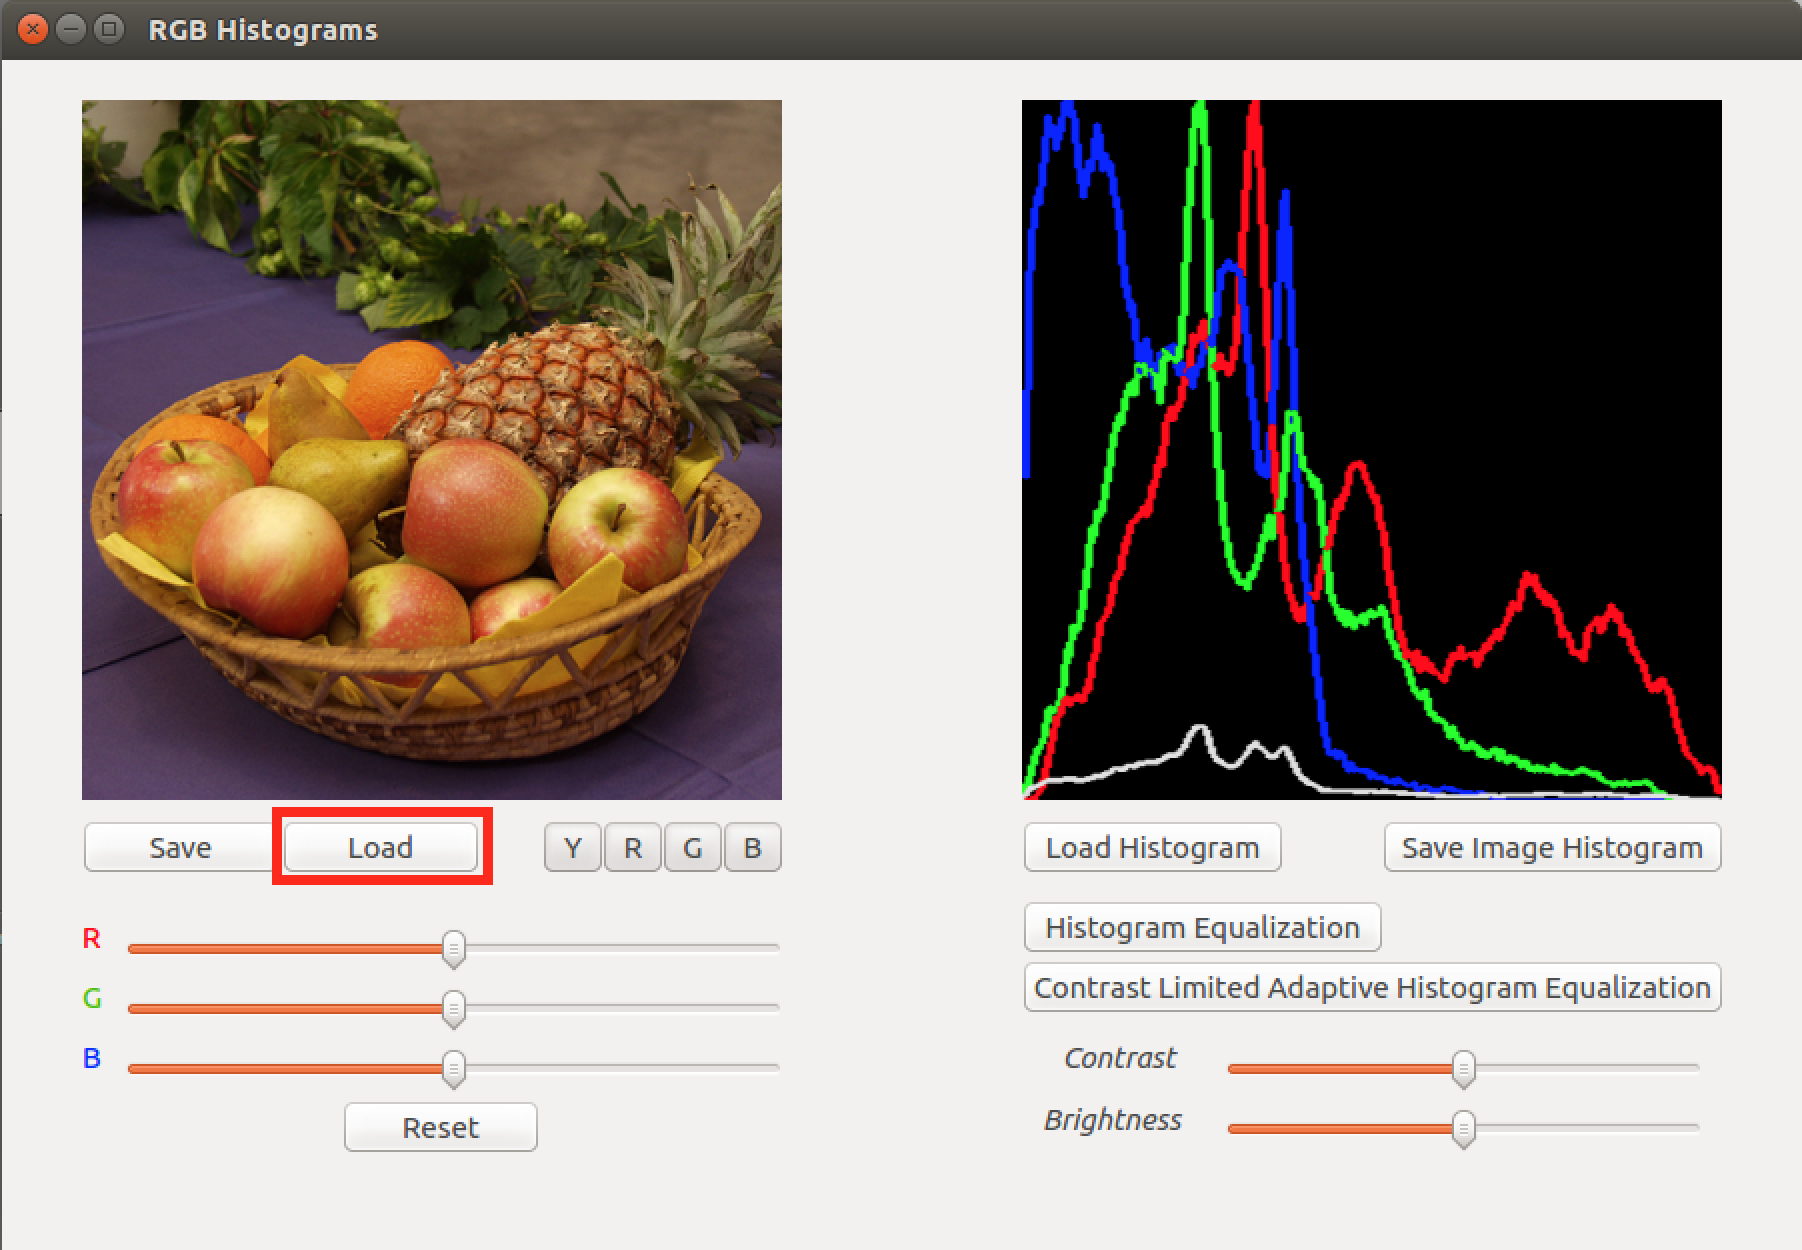
\includegraphics[width=60mm,scale=1]{imagens/window_load.png}
 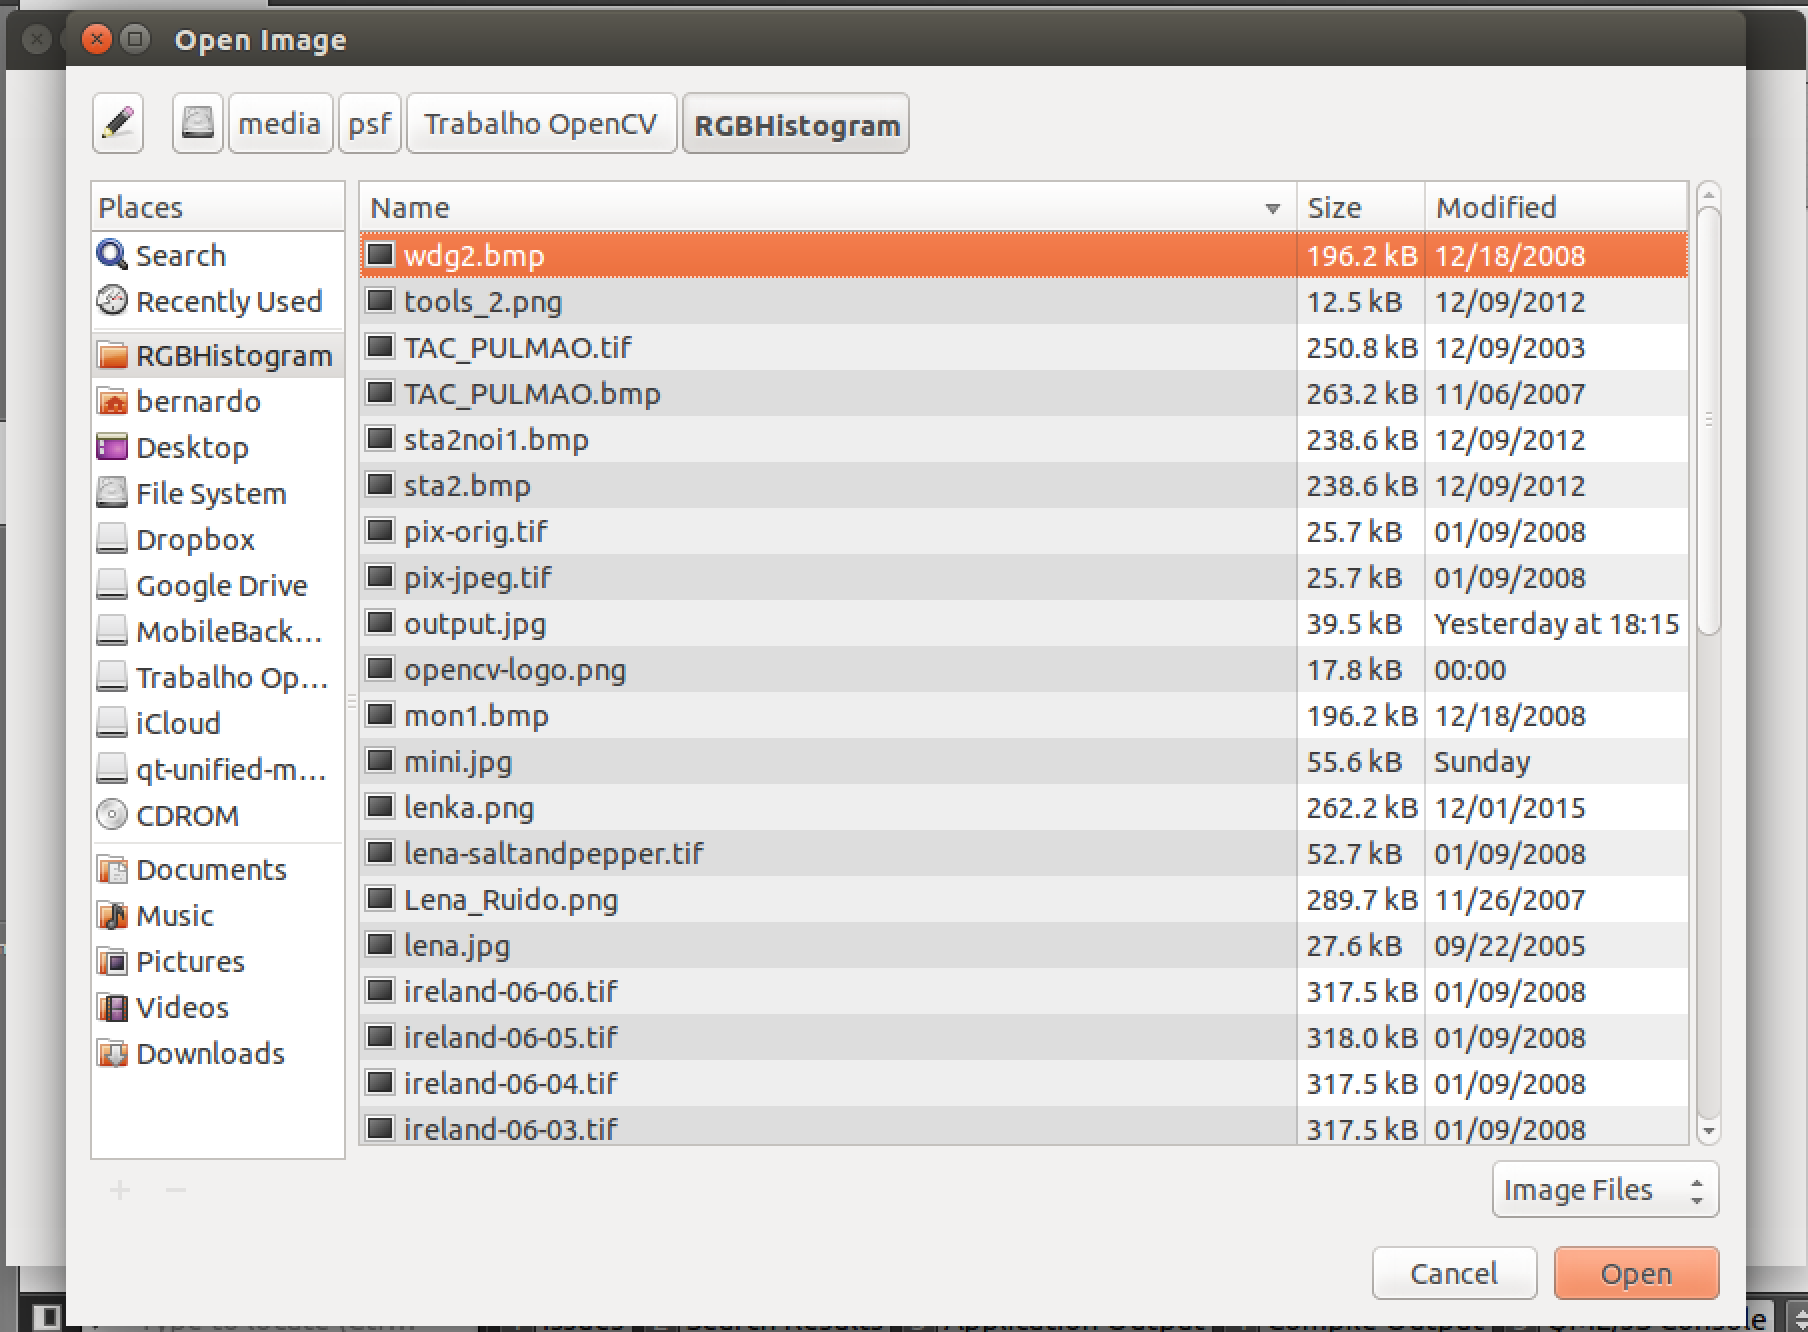
\includegraphics[width=60mm,scale=1]{imagens/window_open_image.png}
 \caption{Abrir uma nova imagem}
 \label{fig:open_book}
\end{figure}

Para abrir uma nova imagem o utilizador deve clicar em "Load". Irá aparecer uma janela que permitirá escolher uma imagem dos seguintes formatos: *.png, *.jpg, *.bmp, *.tif. Após isso irá aparecer uma nova janela com a nova imagem.

\newpage

\subsection{Visualizar as diferentes componentes RGB}

\begin{figure}[!htb]
\center
 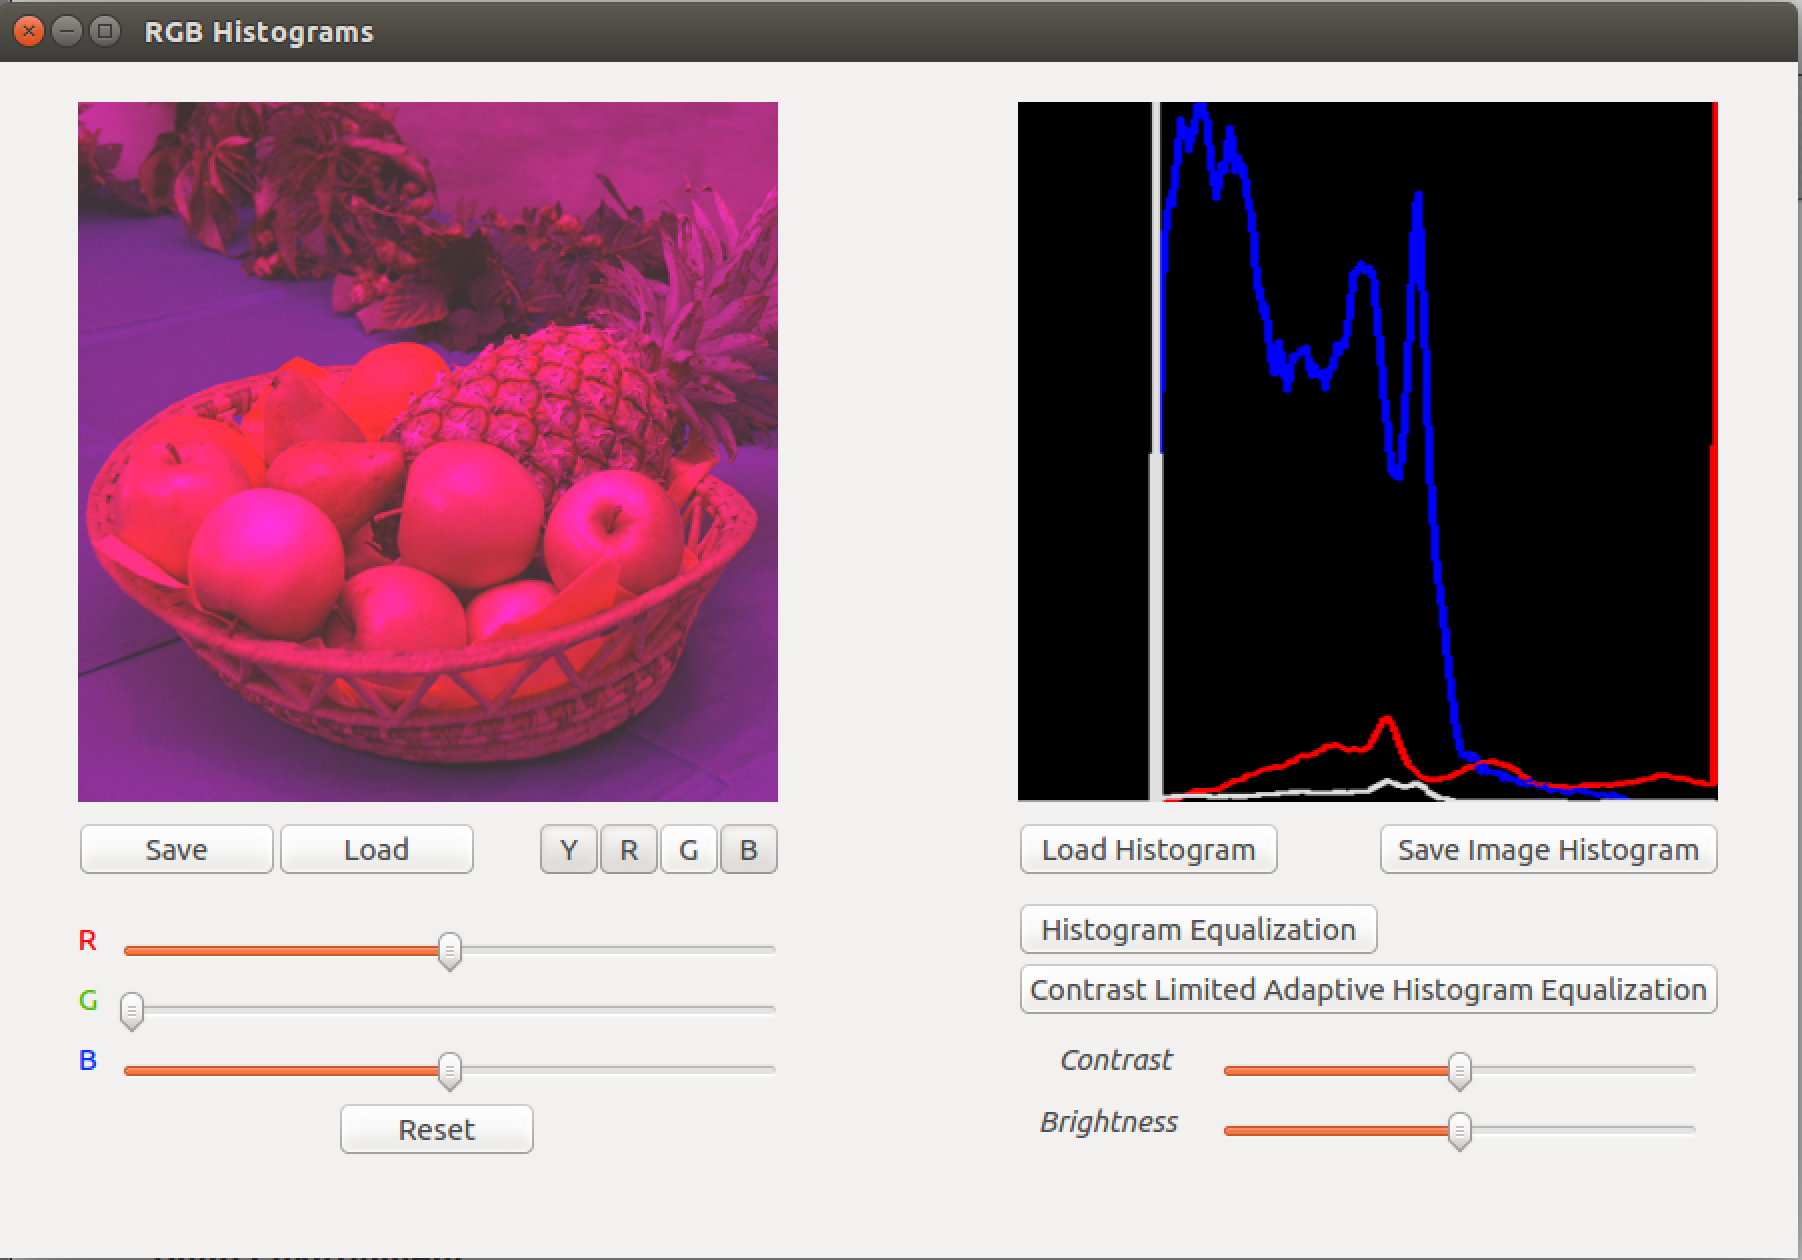
\includegraphics[width=60mm,scale=1]{imagens/without_green.png}
 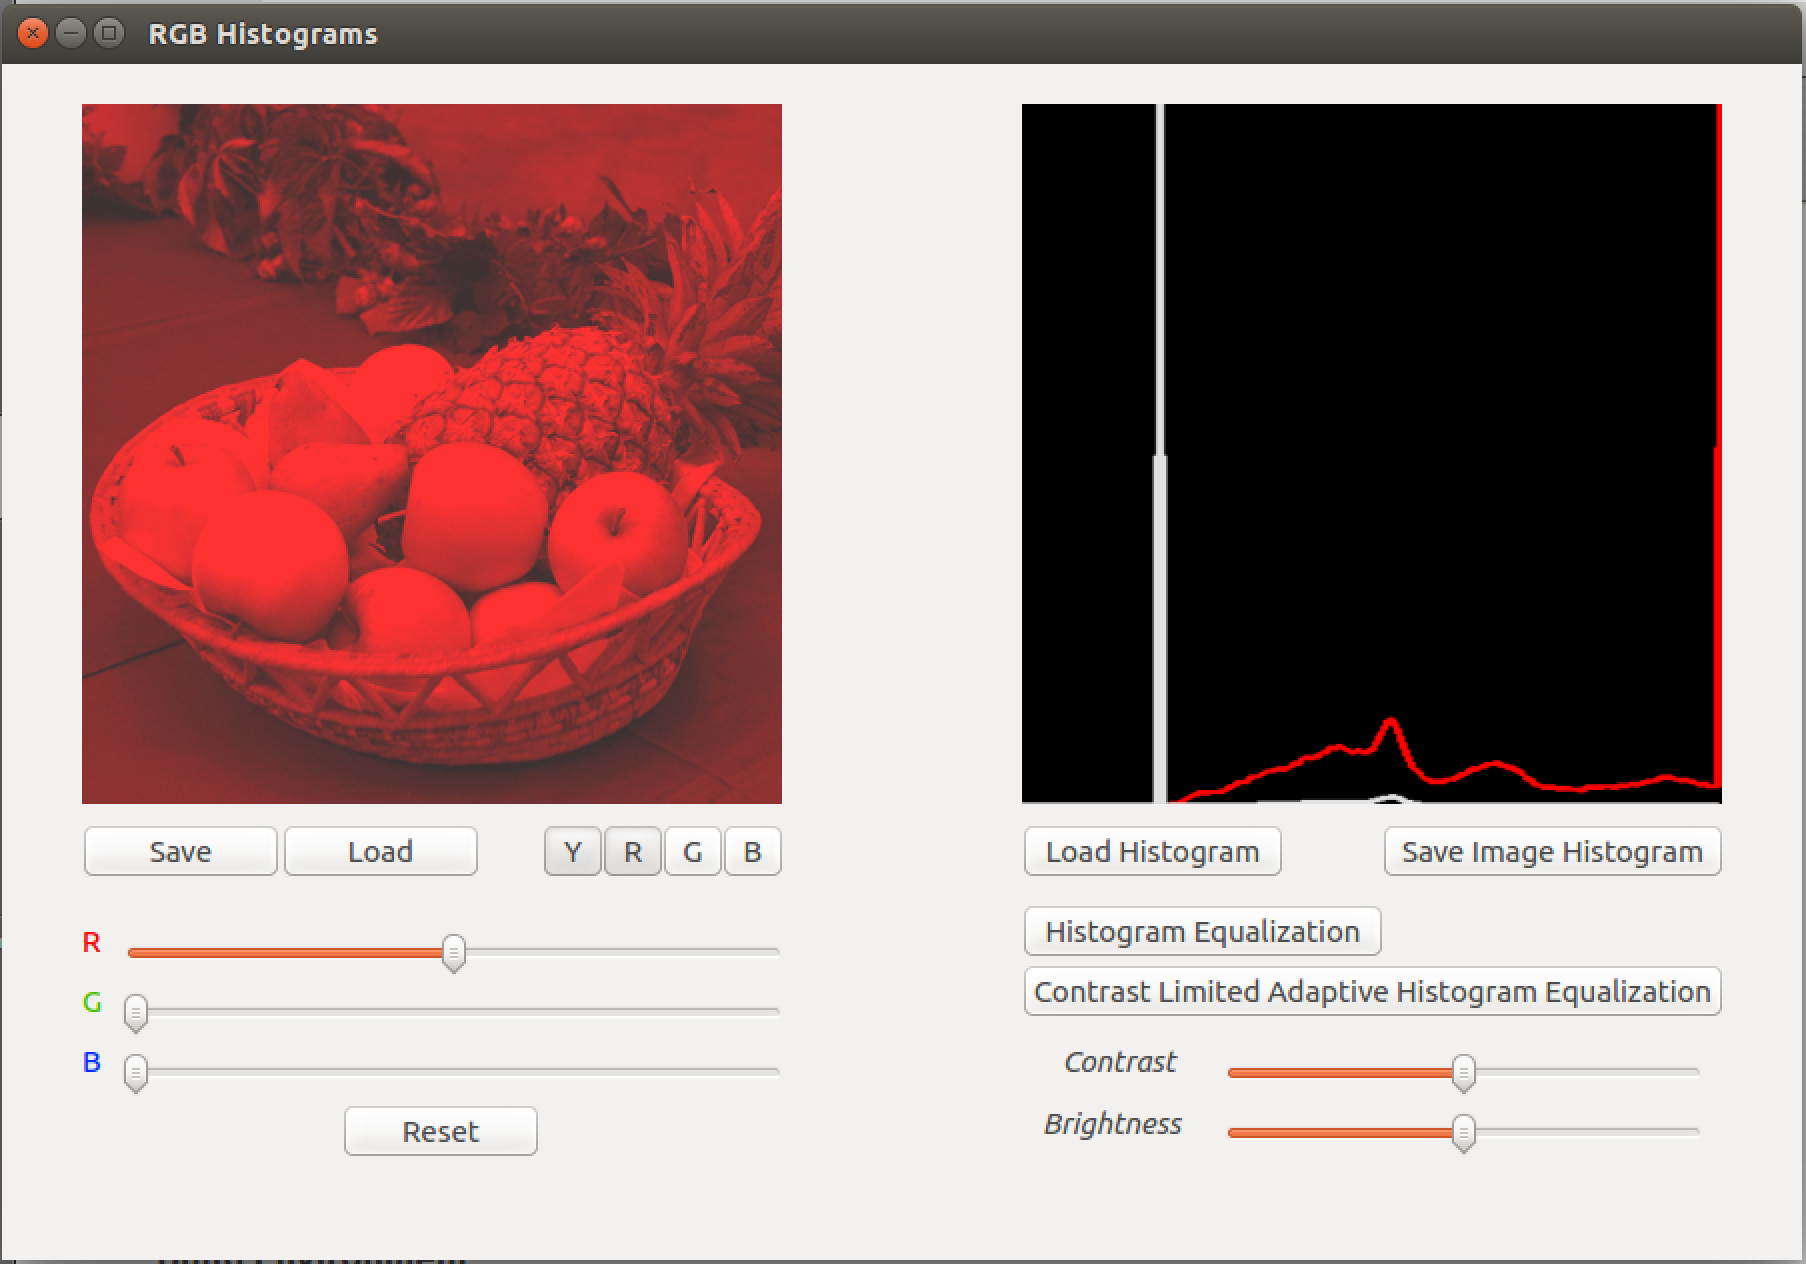
\includegraphics[width=60mm,scale=1]{imagens/only_red.png}
 \caption{Visualizar as diferentes componentes de forma separada}
 \label{fig:select_components}
\end{figure}

Foi dada a possibilidade ao utilizador de selecionar as componentes que pretende visualizar, assim como os histogramas das mesmas. Nos botões "R", "G", "B", que são do tipo "checkable", se estiverem selecionados irá ser apresentado a componente correspondente, sempre que não estiverem selecionados, essa componente não irá aparecer.

Por exemplo, na primeira imagem da figura \ref{fig:select_components}, apenas estão selecionadas as componentes vermelho e azul e por isso a componente verde não aparece nem na imagem, nem no histograma.

Na segunda imagem da mesma figura, apenas está selecionada a componente vermelha, sendo que apenas esta aparece na imagem e no histograma.

\subsubsection{Implementação}
Para implementação do histograma com as diferentes componentes foi usado um tutorial\footnote{\label{url2} \url{http://docs.opencv.org/2.4/doc/tutorials/imgproc/histograms/histogram_calculation/histogram_calculation.html?highlight=histogram}} do OpenCV que explica como se deve dividir as diferentes componentes e criar assim histogramas para cada uma.

\subsection{Visualizar apenas a Luminância}

\begin{figure}[!htb]
\center
 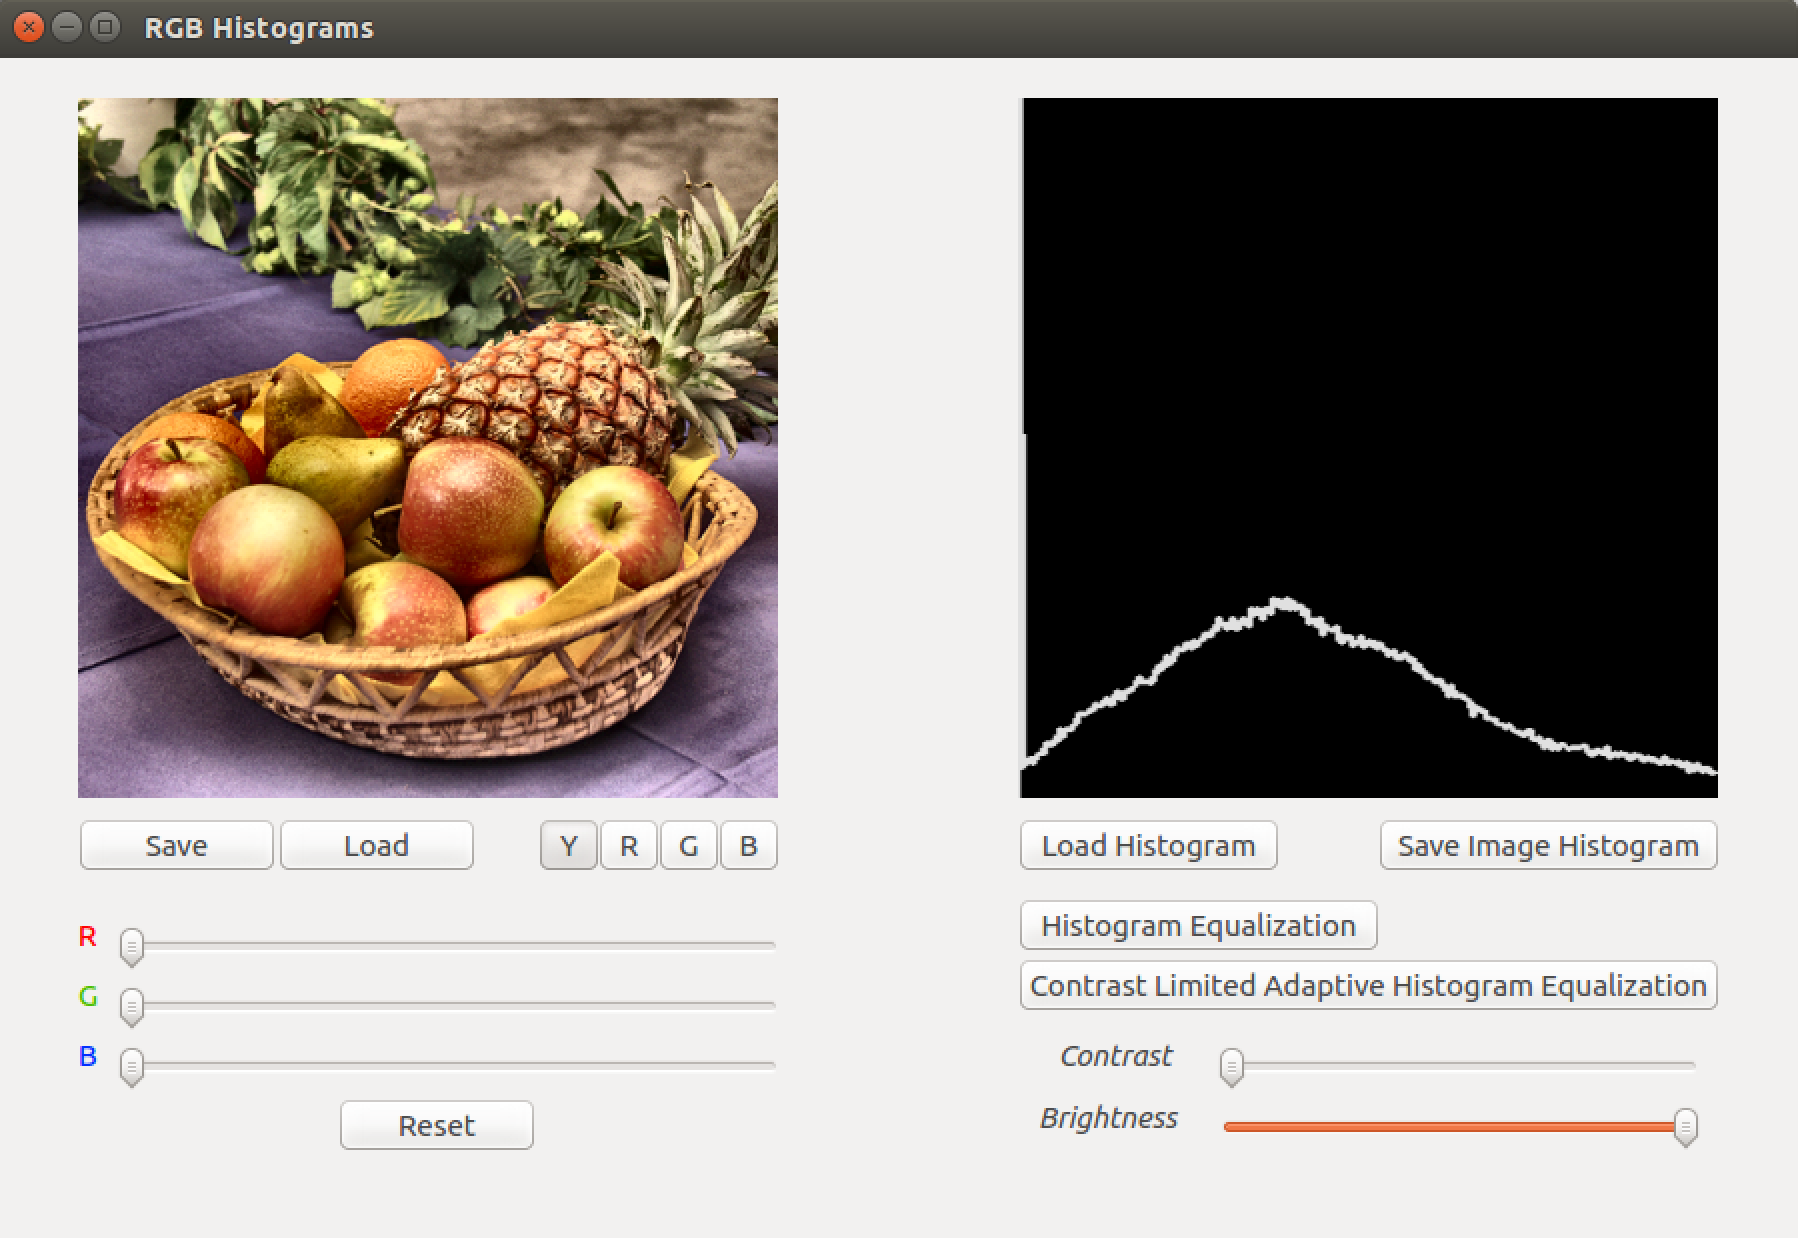
\includegraphics[width=60mm,scale=1]{imagens/only_brightness.png}
 \caption{Visualizar apenas a luminância num histograma}
\end{figure}

O utilizador pode também apenas visualizar a luminância para uma determinada imagem. Para isso, tem de não selecionar os botões vermelho, verde e azul. Sendo assim, apenas o botão da luminância fica selecionado, aparecendo assim no histograma apenas a luminância.

\subsubsection{Implementação}
Para determinar a luminância\footnote{\label{url3} \url{http://www.programming-techniques.com/2013/01/intensity-histogram-using-c-and-opencv.html}} foi criado um array com 256 entradas para guardar cada valor de intensidade e inicializados a zero. Depois foram calculados o número de pixeis para cada valor de intensidade. De seguida foi encontrado o valor máximo de intensidade do histograma e foi também normalizado o histograma entre 0 e o número de linhas do histograma.

\subsection{Guardar uma imagem ou um histograma}

\begin{figure}[!htb]
\center
 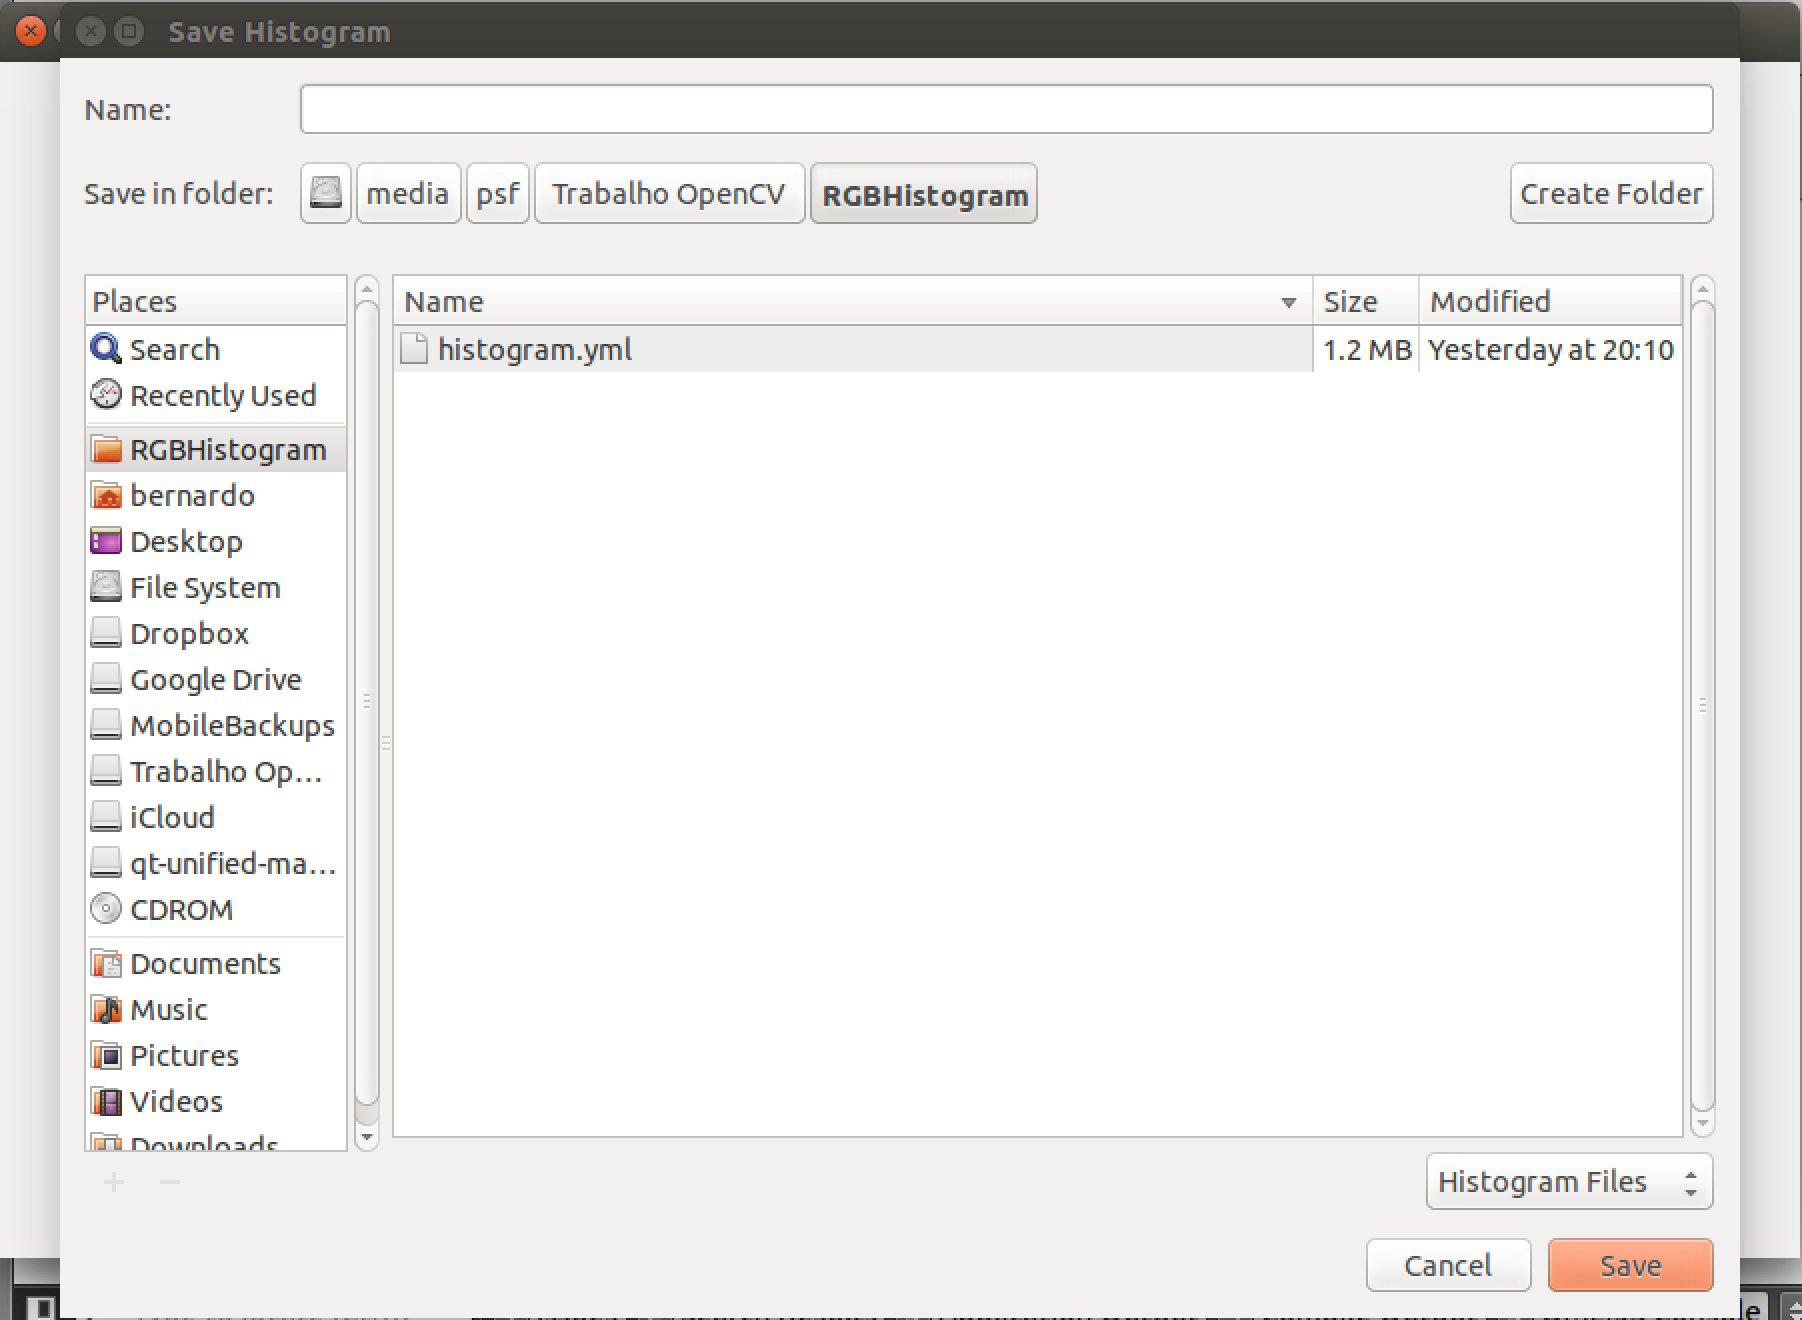
\includegraphics[width=60mm,scale=1]{imagens/save_histogram.png}
 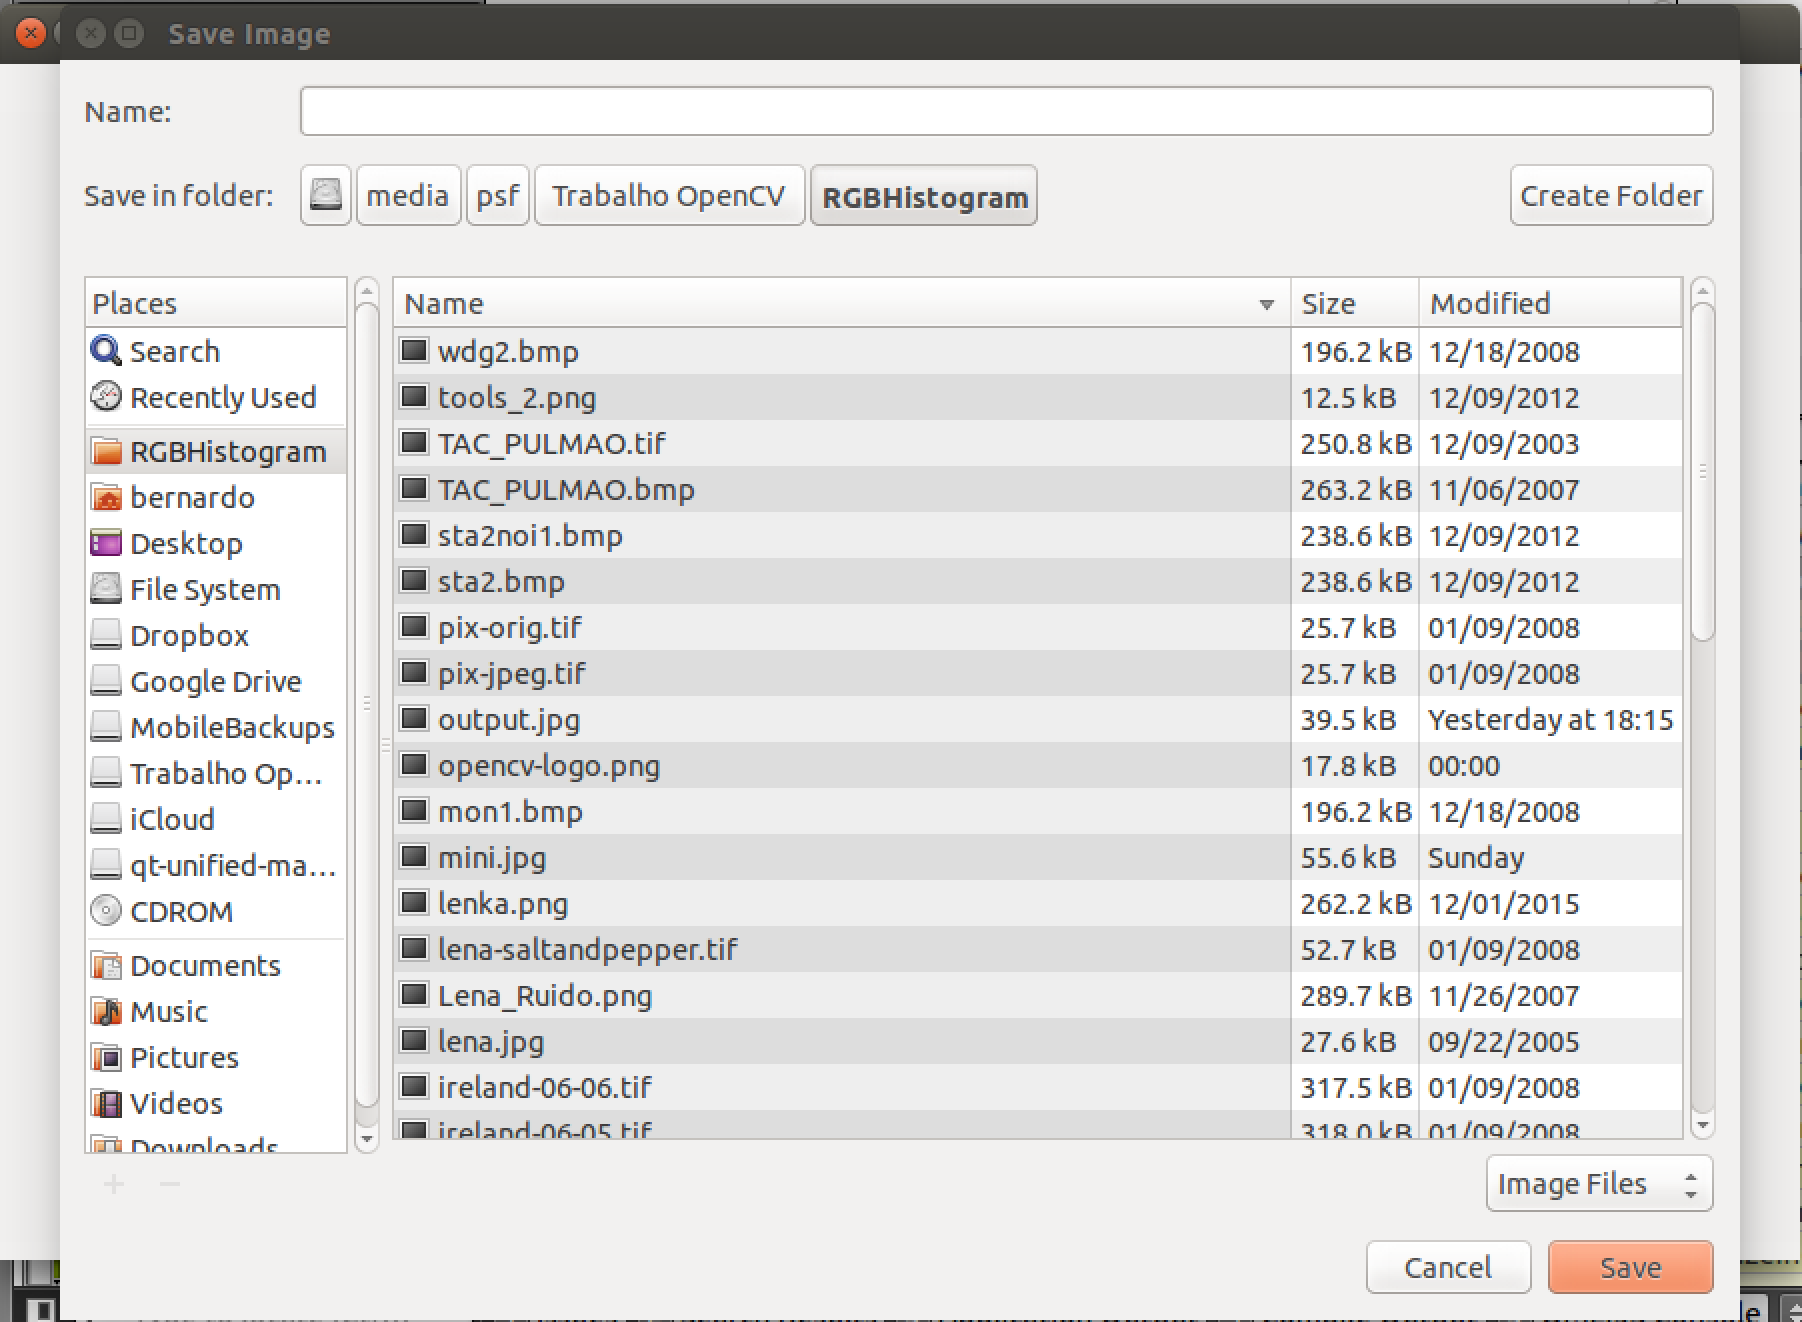
\includegraphics[width=60mm,scale=1]{imagens/save_image.png}
 \caption{Janelas para o utilizador guardar uma imagem ou histograma}
 \label{fig:save_images}
\end{figure}

O utilizador pode exportar as imagens em diferentes formatos (*.png, *.jpg, *.bmp, *.tif) e guardar o histograma no formato *.yml\footnote{\label{url4} \url{http://stackoverflow.com/questions/10277439/opencv-load-save-histogram-data}}.

\newpage

\subsection{Abrir um novo histograma para comparação}

\begin{figure}[!htb]
\center
 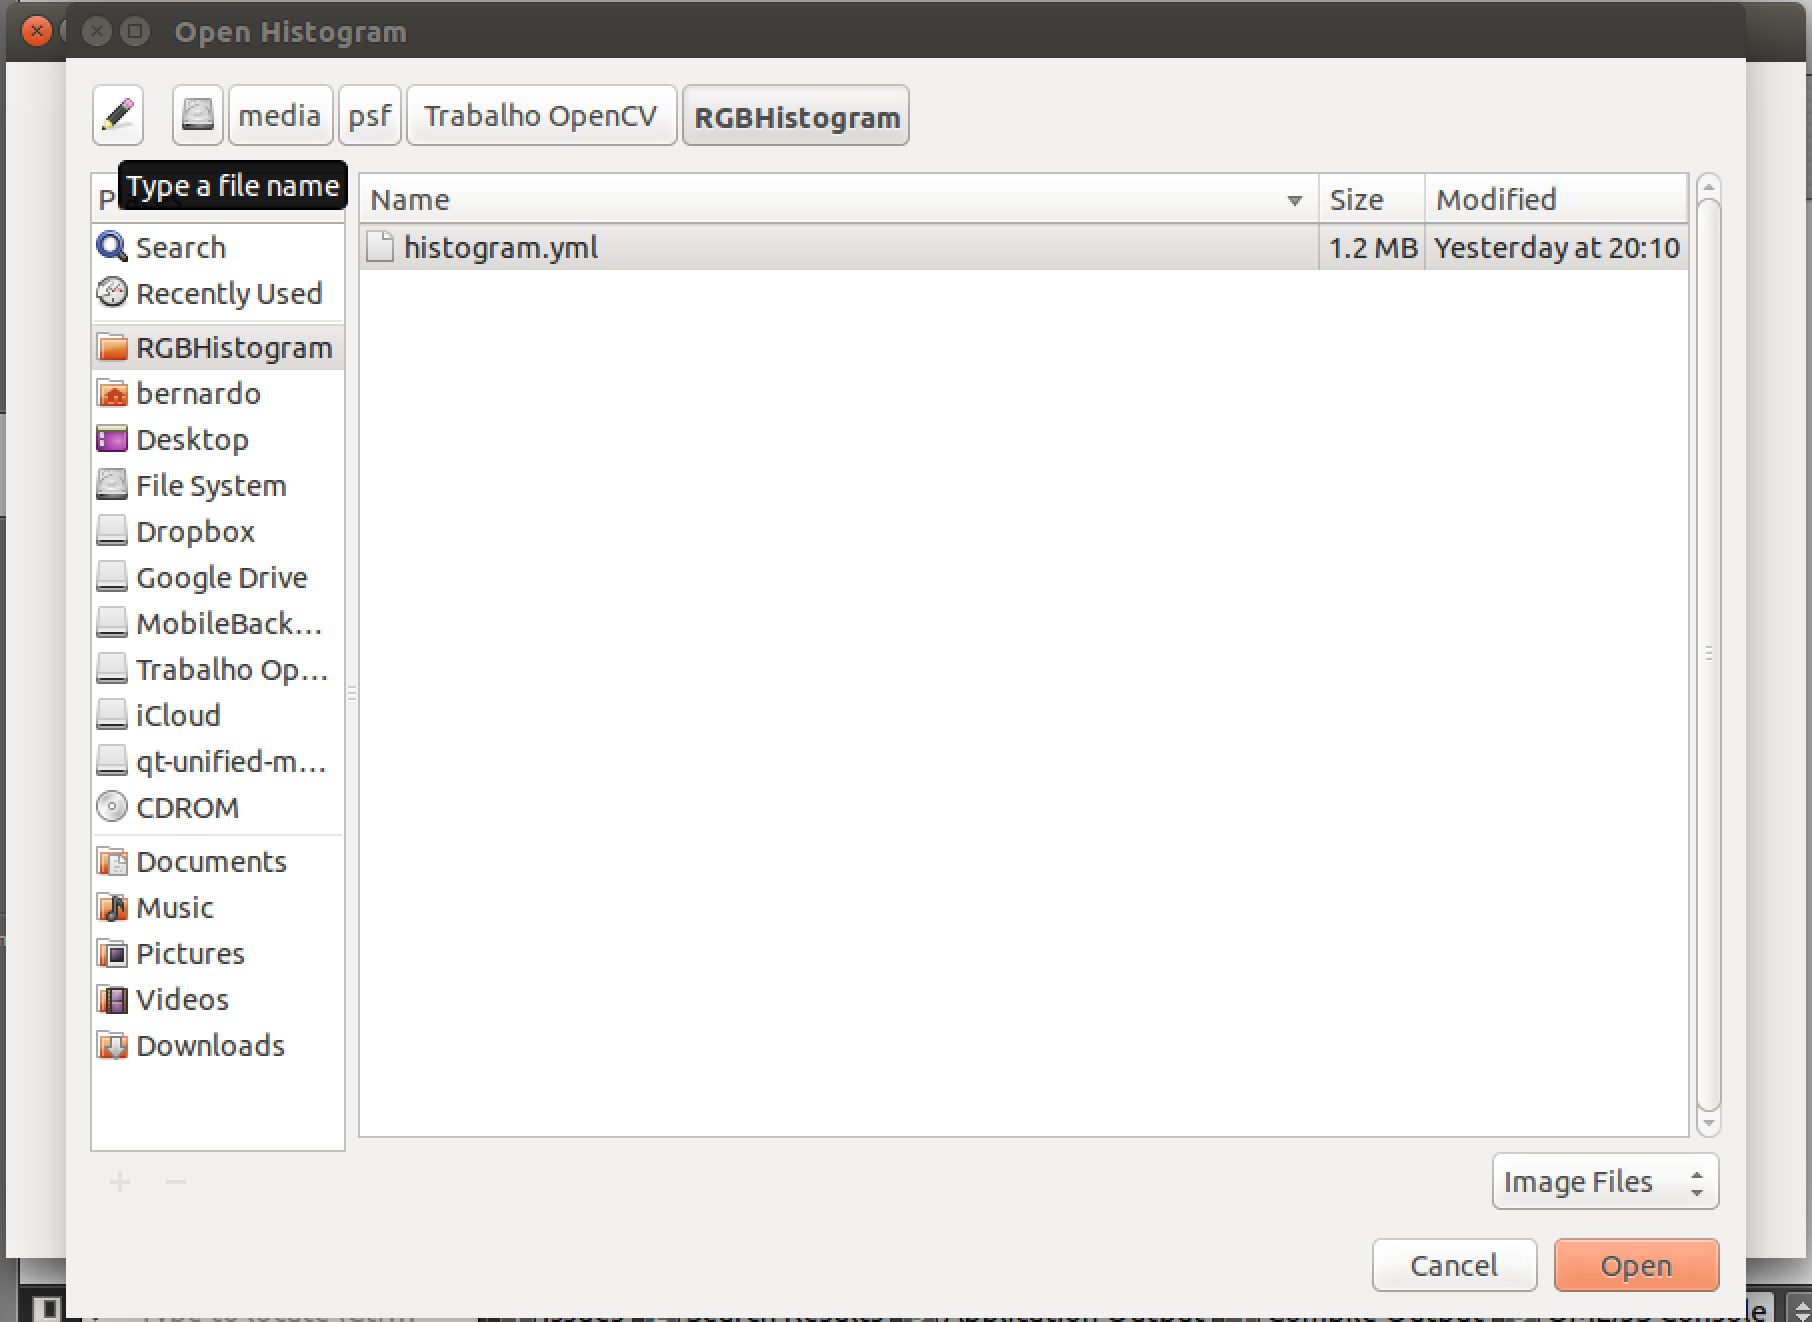
\includegraphics[width=60mm,scale=1]{imagens/open_histogram.png}
 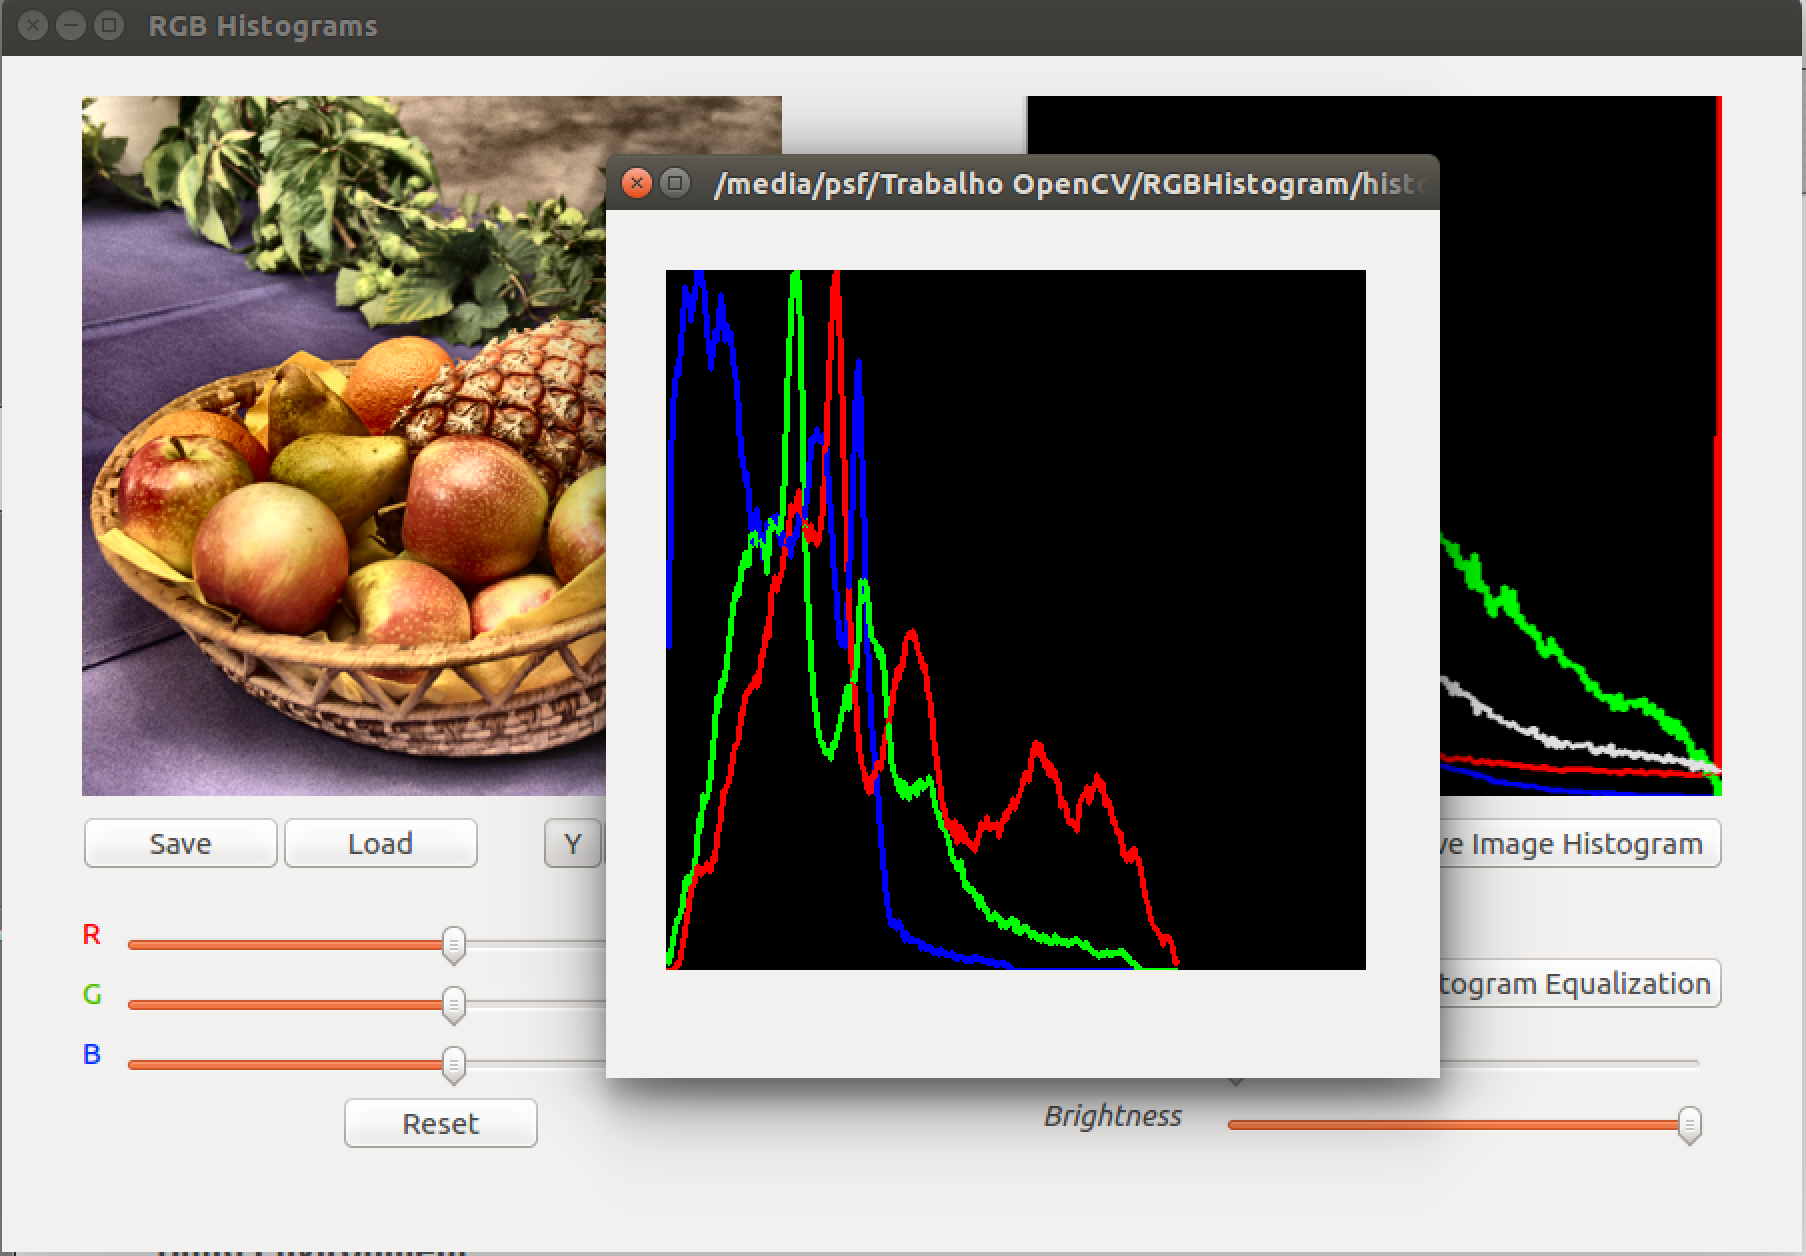
\includegraphics[width=60mm,scale=1]{imagens/see_histogram.png}
 \caption{O utilizador abre o histograma numa nova janela}
 \label{fig:save_images}
\end{figure}

Foi dada a possibilidade de o utilizador abrir um histograma numa nova janela para conseguir comparar esse histograma com o que está a ser mostrado na imagem aberta na janela principal.

\subsection{Mudar o contraste da imagem}

\begin{figure}[!htb]
\center
 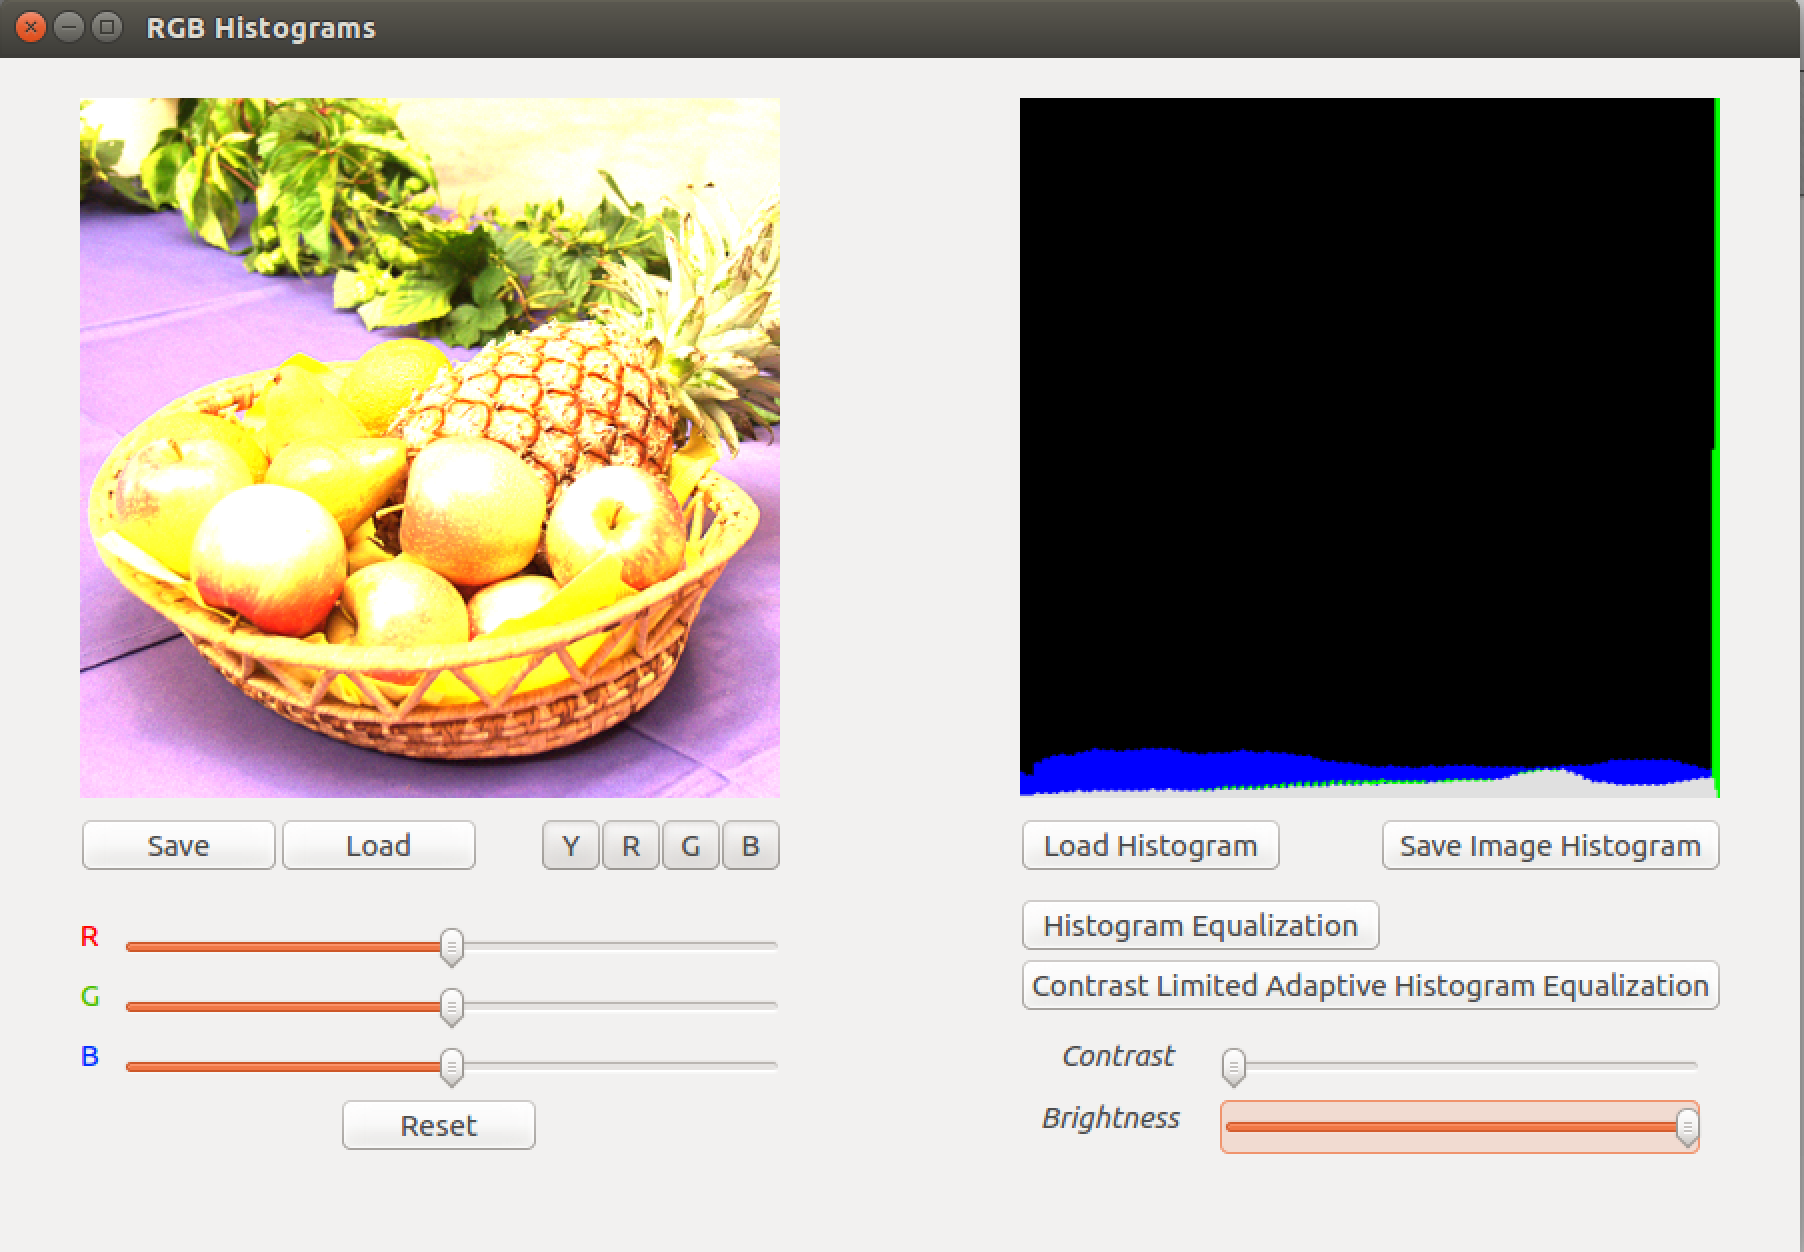
\includegraphics[width=60mm,scale=1]{imagens/maximum_contrast.png}
 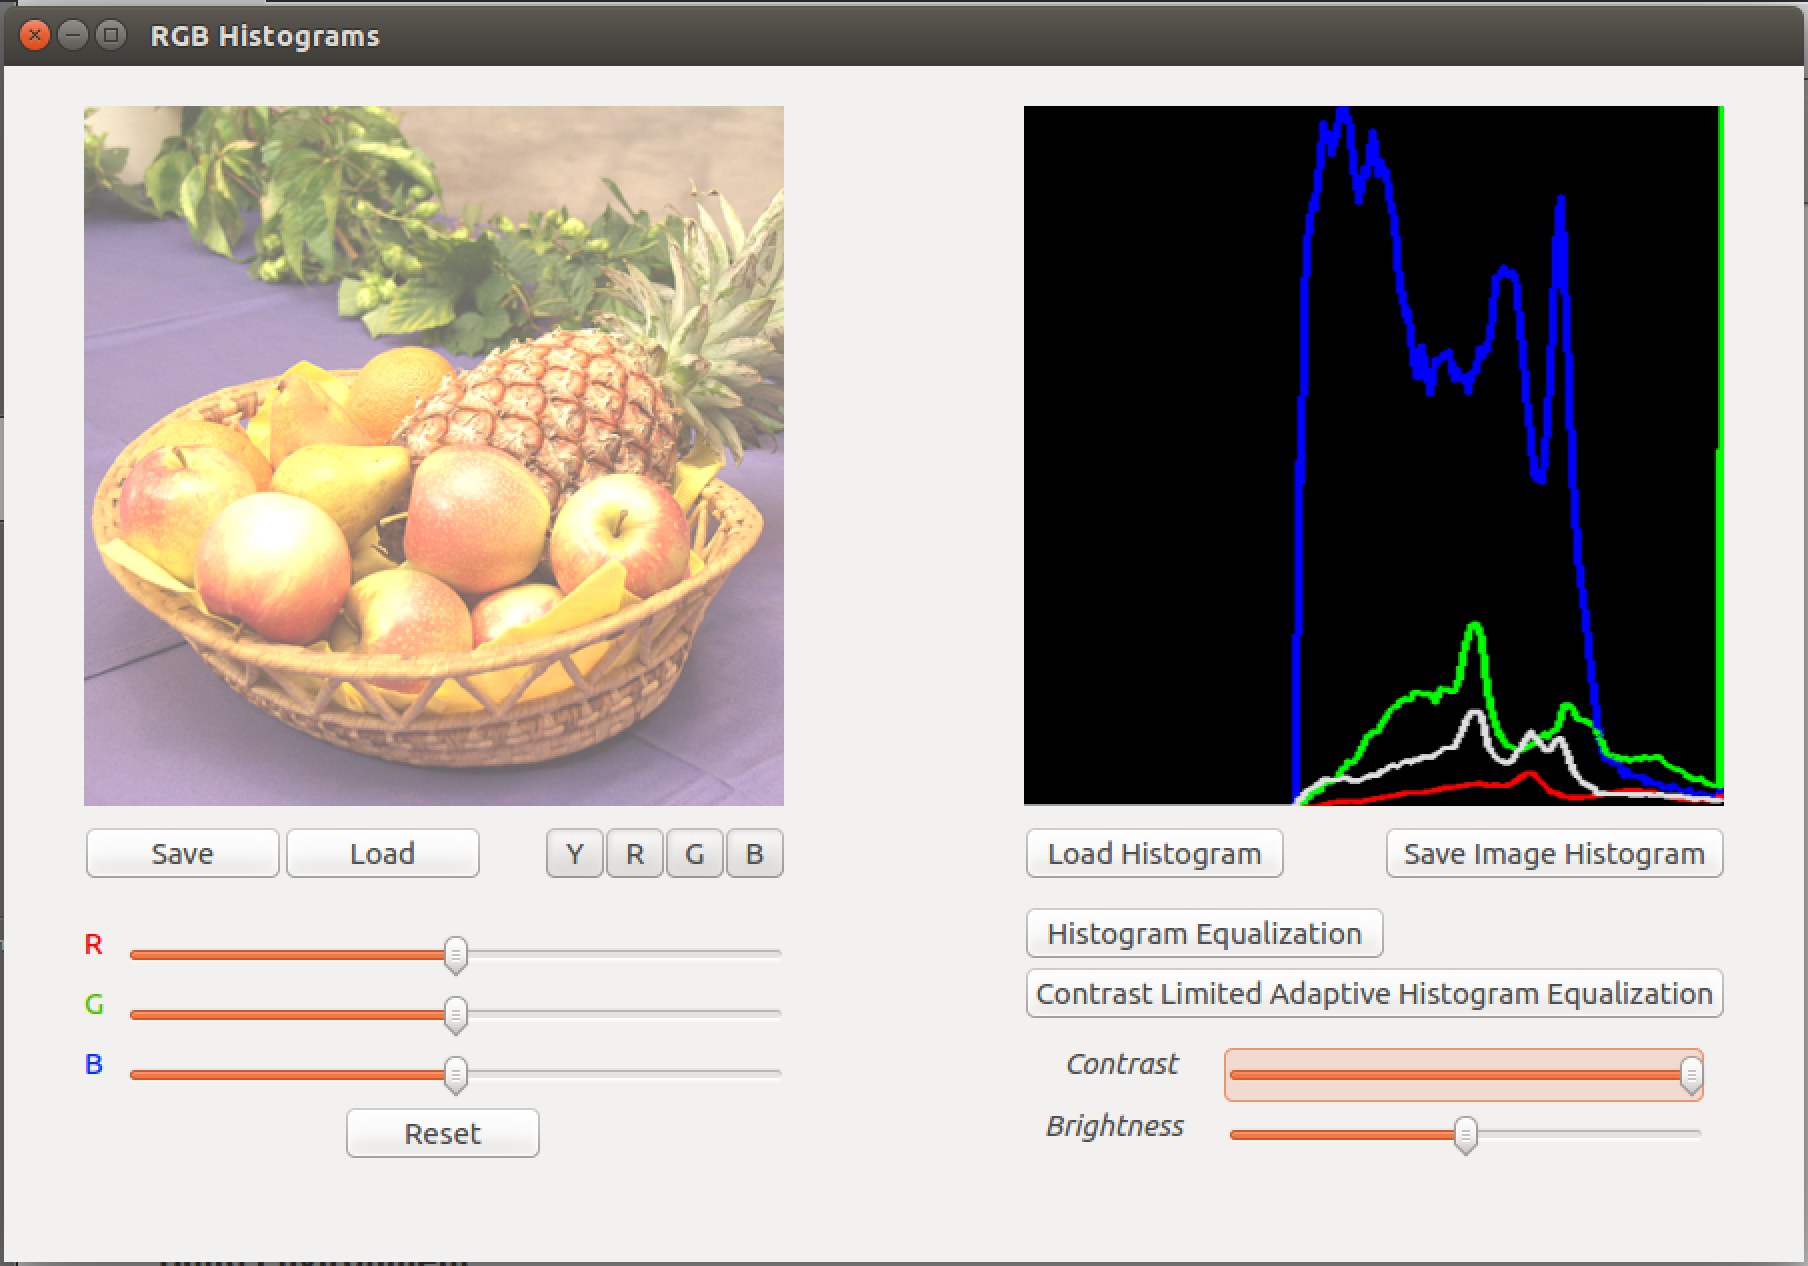
\includegraphics[width=60mm,scale=1]{imagens/high_contrast.png}
 \caption{Mudar o contraste usando os sliders}
 \label{fig:contrastes}
\end{figure}

Caso o utilizador pretenda, pode alterar o contraste da imagem, por exemplo, na figura \ref{fig:contrastes} o utilizador pode selecionar qual o contraste que a imagem apresenta, se o máximo, se o mínimo contraste ou outro valor.

\newpage

\subsection{Mudar o brilho da imagem}

\begin{figure}[!htb]
\center
 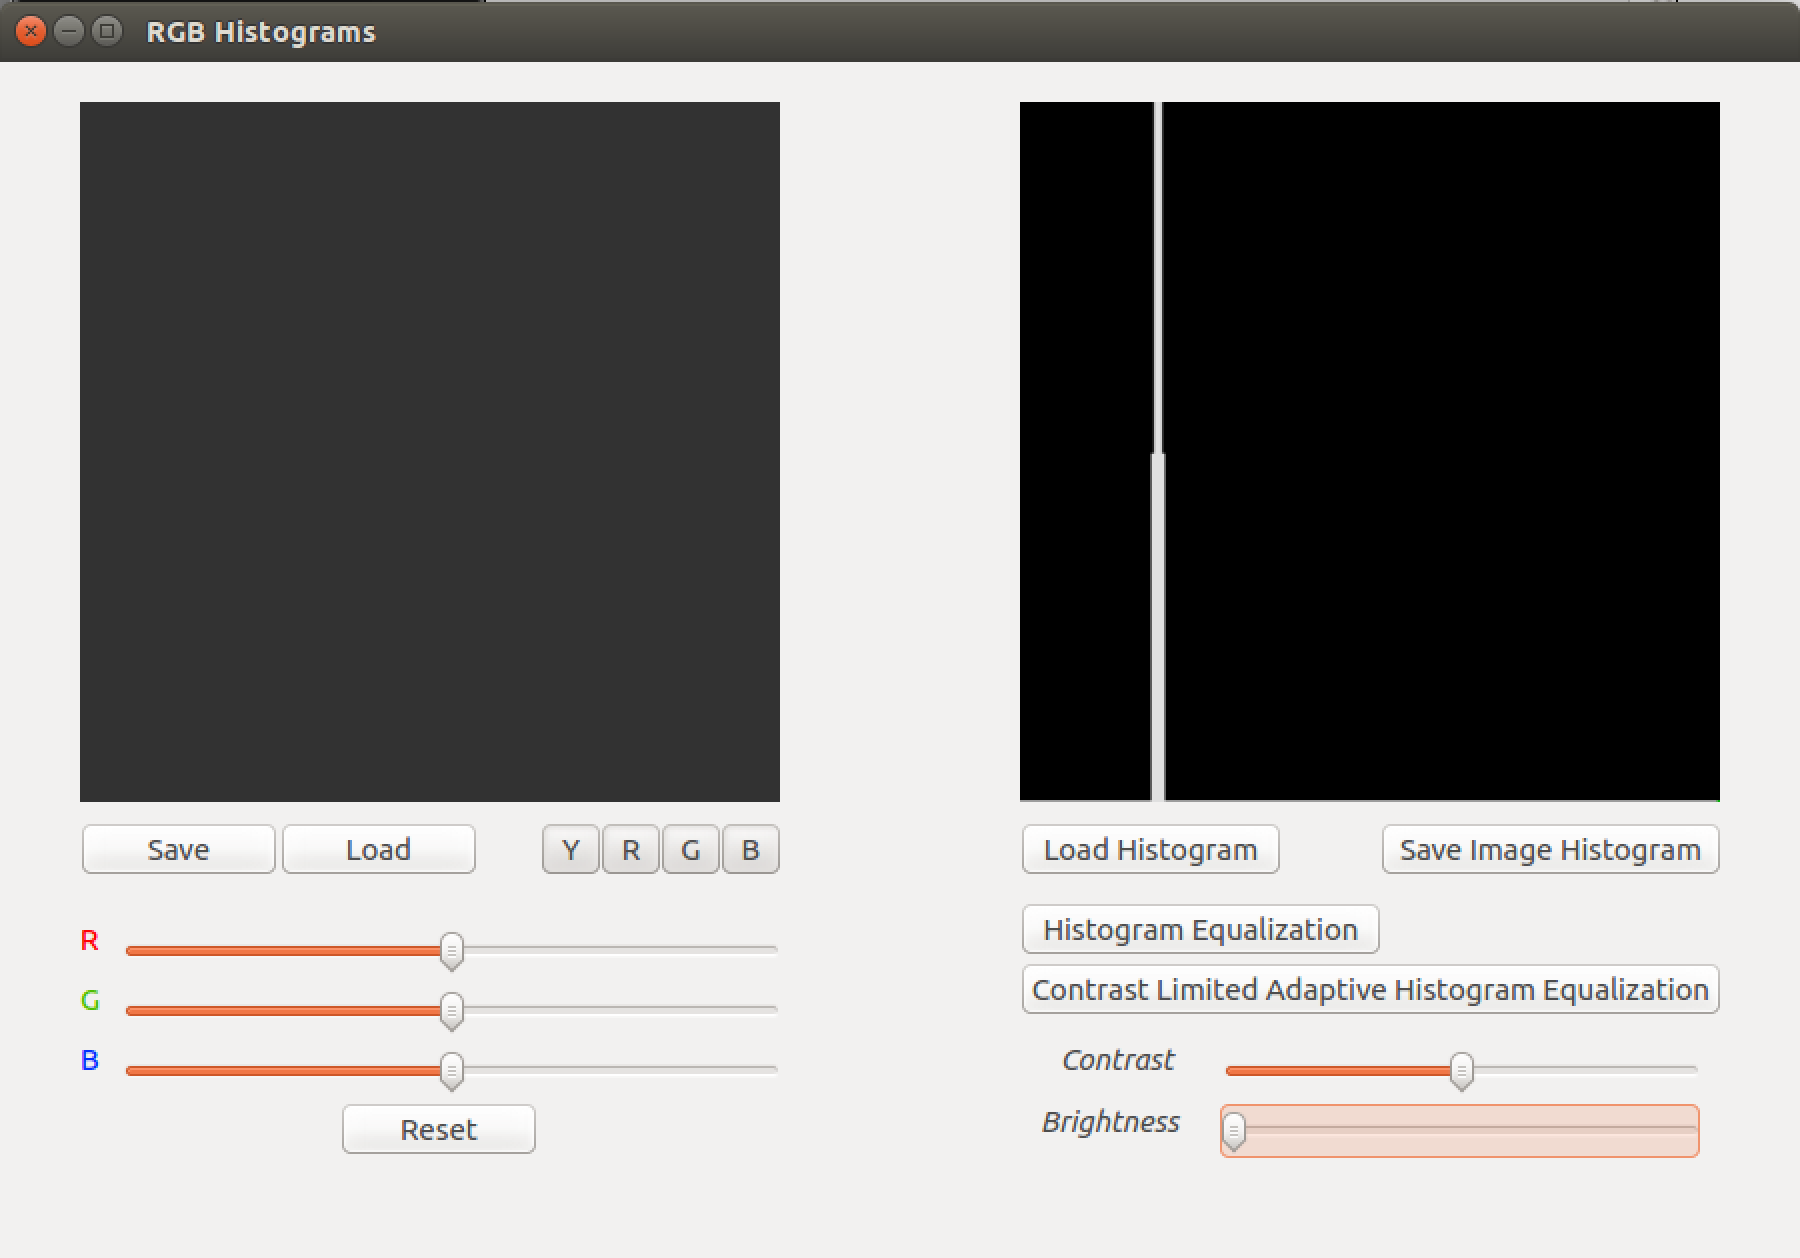
\includegraphics[width=60mm,scale=1]{imagens/low_brigh.png}
 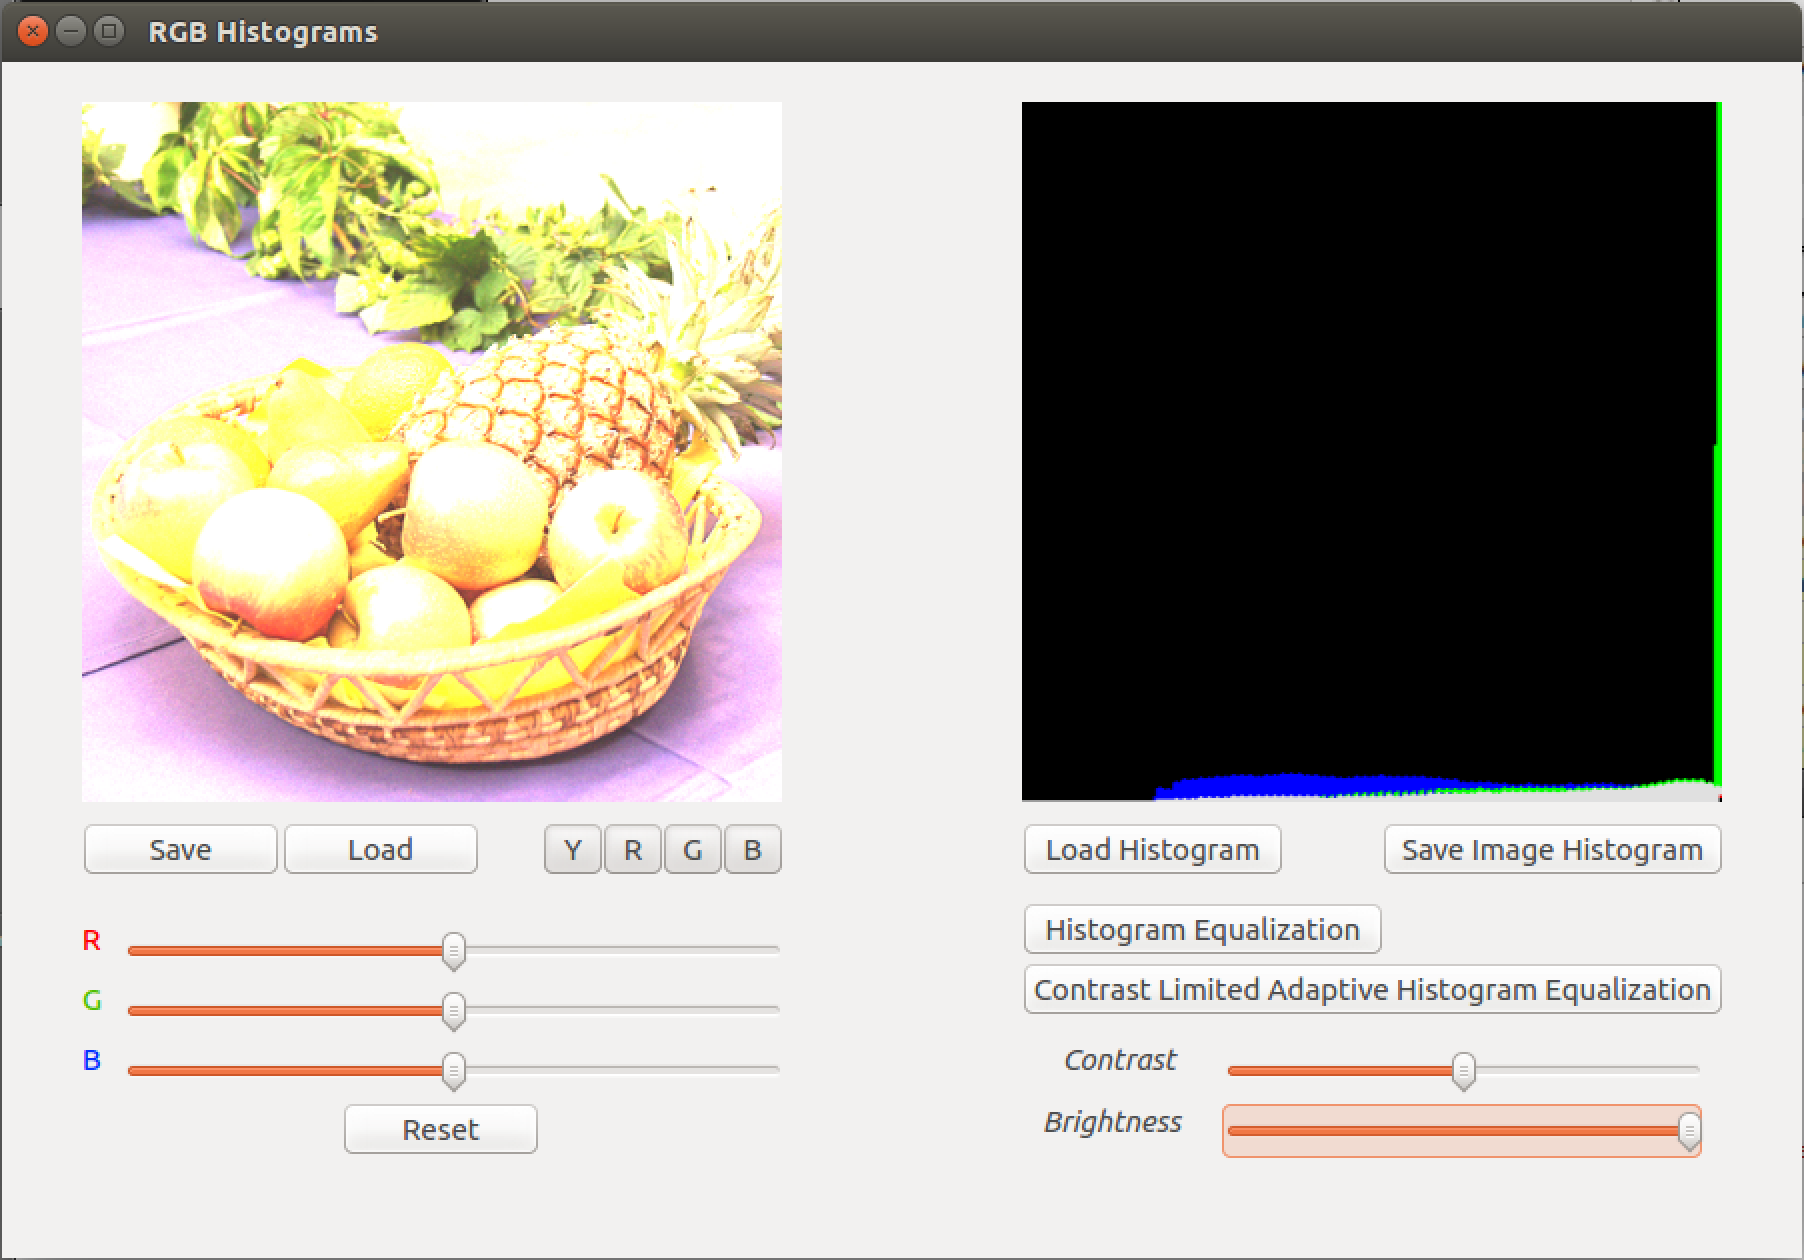
\includegraphics[width=60mm,scale=1]{imagens/high_brigh.png}
 \caption{Mudar o brilho usando os sliders}
 \label{fig:brilho}
\end{figure}

Também foi dada a possibilidade para que caso o utilizador pretenda, possa alterar o brilho da imagem, por exemplo, na figura \ref{fig:brilho} o utilizador pode selecionar qual o brilho que a imagem apresenta, se o máximo, se o mínimo brilho ou outro valor.

\subsection{Contrast Limited Adaptive Histogram Equalization}

\begin{figure}[!htb]
\center
 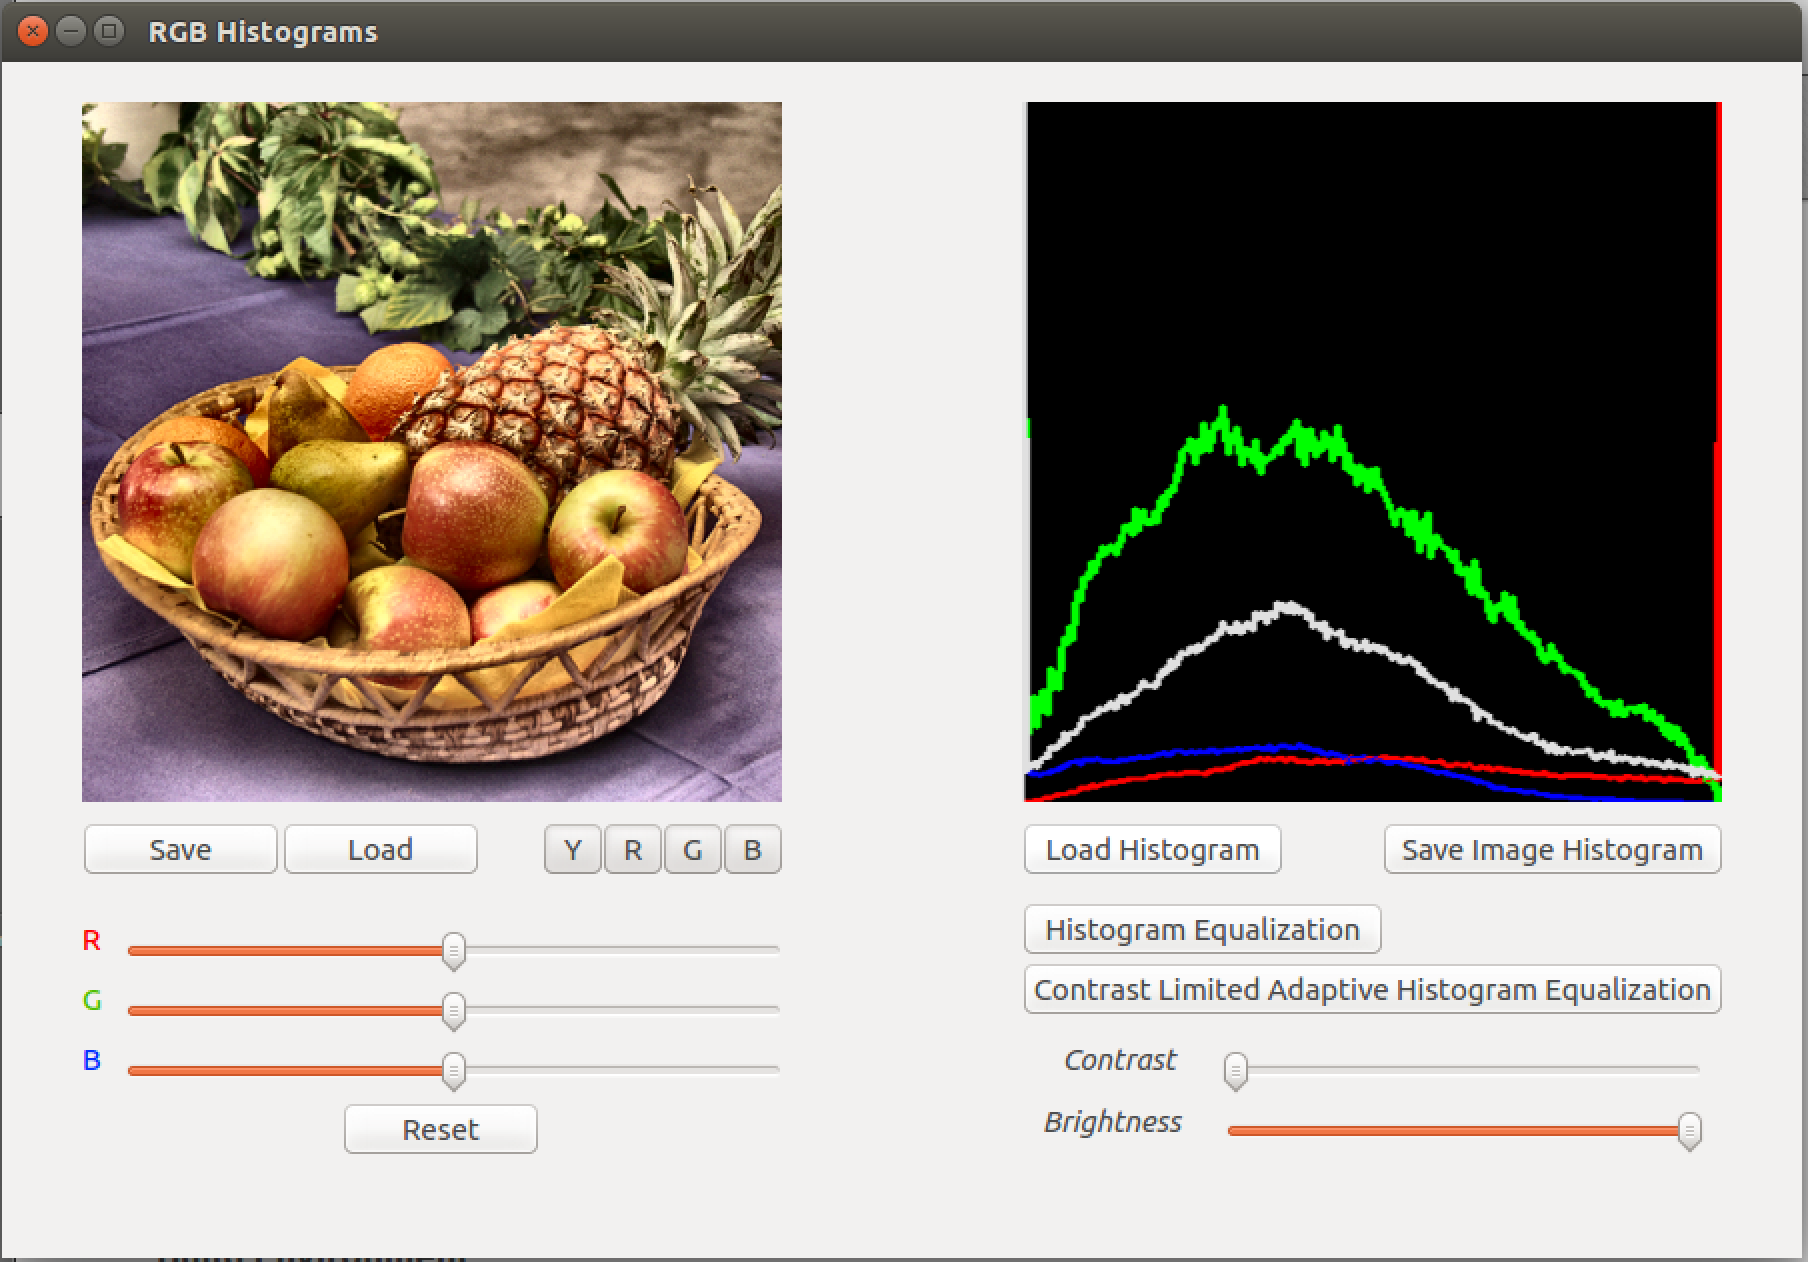
\includegraphics[width=100mm,scale=1]{imagens/window_contrast_limited_ada_contrast.png}
 \caption{Contrast Limited Adaptive Histogram Equalization}
 \label{fig:brilho}
\end{figure}

Para manipulação da imagem e do histograma foi criada uma funcionalidade para o utilizador fazer a equalização do histograma de forma simples. A primeira funcionalidade\footnote{\label{url5} \url{http://docs.opencv.org/master/d5/daf/tutorial_py_histogram_equalization.html}} foi a "Contrast Limited Adaptive Histogram Equalization". 

\subsubsection{Implementação}

A imagem é dividida em pequenos blocos chamados "tiles" e cada desses blocos são depois equalizados de forma igual. Portanto numa pequena área, o histograma vai confinar-se a uma pequena região, se existir ruído, então era ampliar-se. Para evitar isto, é então aplicado "contrast limiting". 

Para esta funcionalidade foi usado código disponível no site do OpenCV, usando o CLAHE.

\subsection{Histogram Equalization}

\begin{figure}[!htb]
\center
 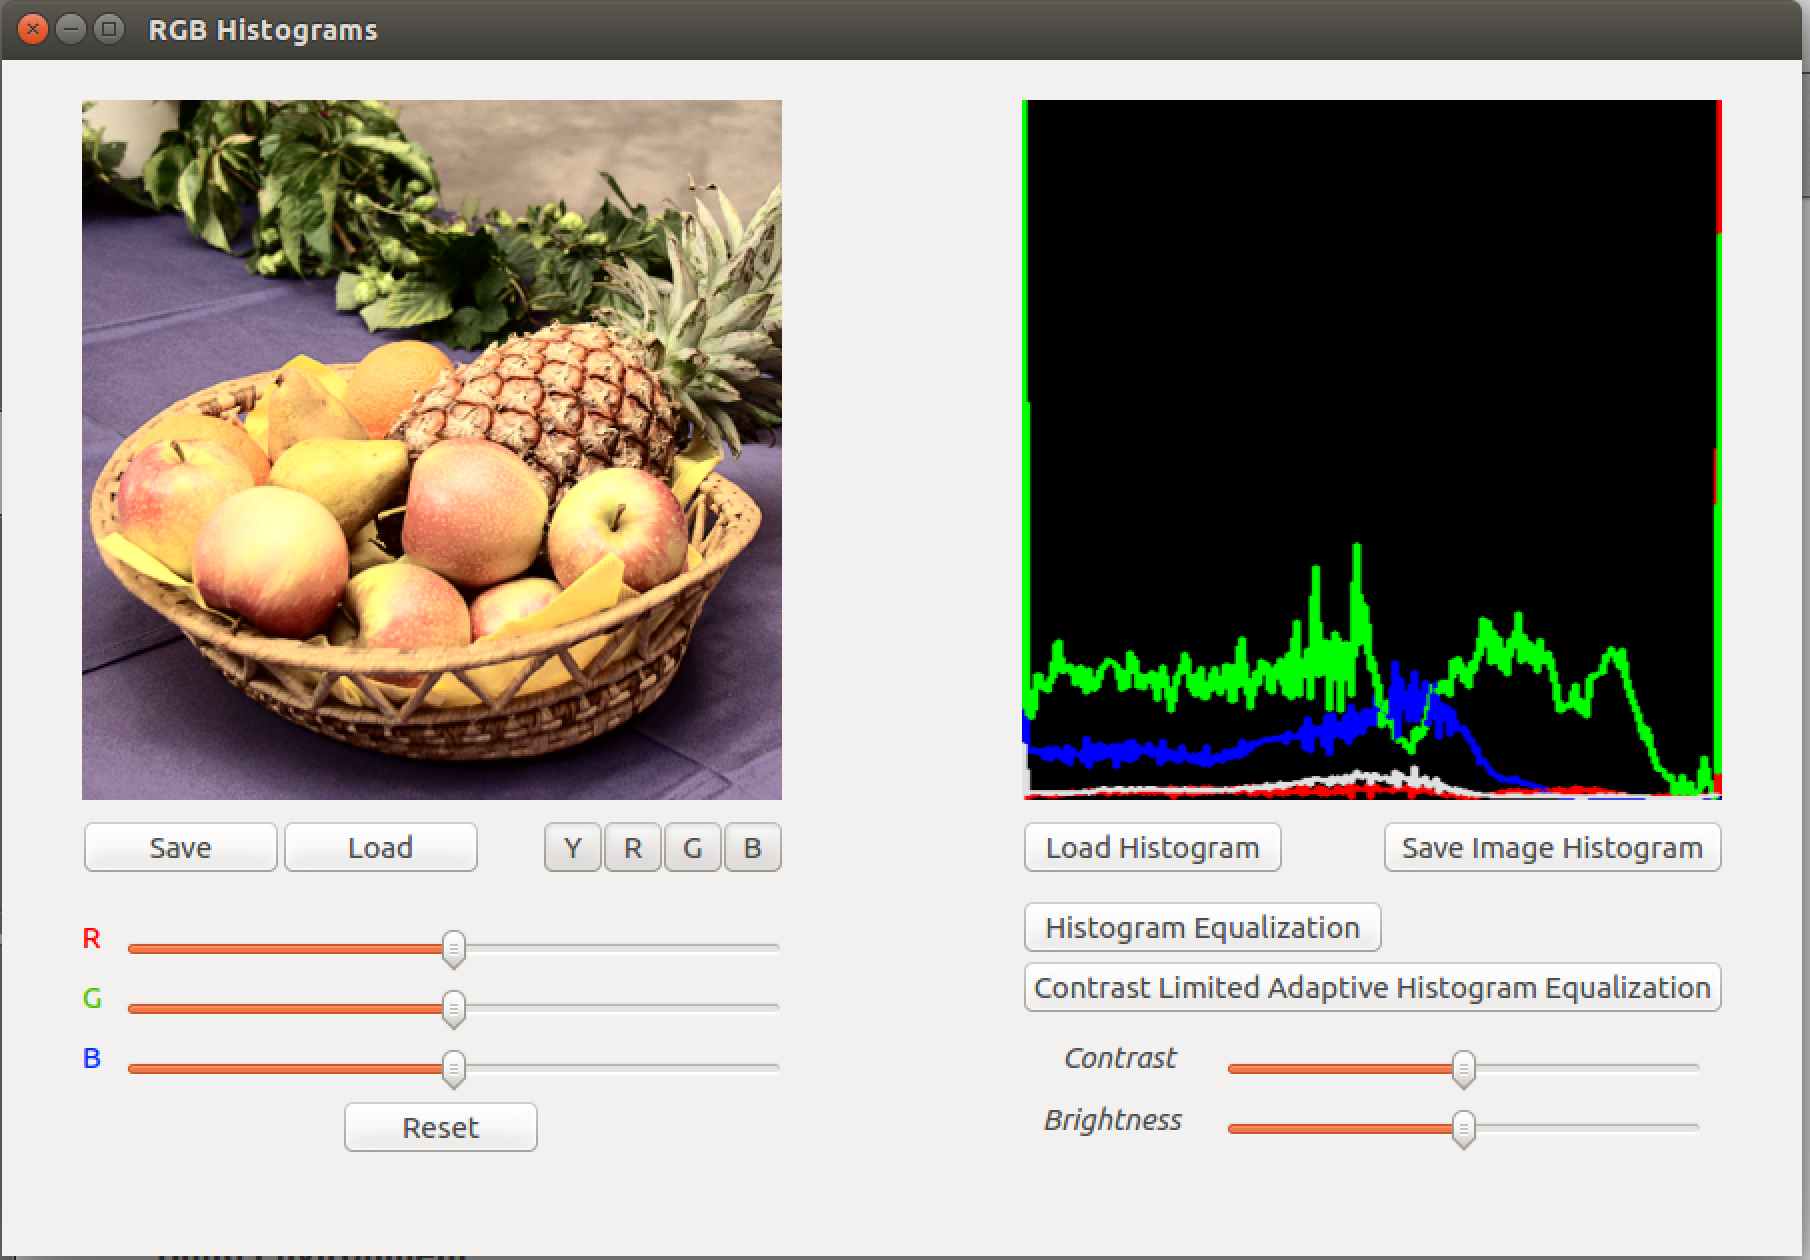
\includegraphics[width=100mm,scale=1]{imagens/histogram_eq.png}
 \caption{Histogram Equalization}
 \label{fig:brilho}
\end{figure}

A outra funcionalidade desenvolvida foi a equalização do histograma RGB. O utilizador, apenas com um clique, consegue equalizar o histograma e visualizar os seus resultados.

\subsubsection{Implementação}

A equalização de um histograma RGB\footnote{\label{url5} \url{http://prateekvjoshi.com/2013/11/22/histogram-equalization-of-rgb-images/}} não pode ser feito da mesma forma que um a preto e branco ou dividindo o R, G e B e equalizar cada uma das componentes, isso seria incorreto. A equalização envolve valores de intensidade da imagem e não pode ser aplicado diretamente à imagem. Necessita-se então de ser aplicada de uma maneira que os valores de intensidade são equalizados de maneira a que não modifiquem as cores da imagem. Portanto, o primeiro passo é converter a imagem RGB para um formato que tenha mais valores sobre a intensidade e os separe, por exemplo HSV/HLS, YUV, YCbCr. Escolheu-se então o YCbCR porque está desenhado para imagens digitais. Depois de equalizado converte-se novamente para RGB.

\section{Conclusão}

O principal objetivo foi conseguido, inicialmente teve-se um pouco de receio ao usar Qt, devido à inexperiência com o mesmo e a dificuldade que se sentiria ao juntar o Qt e o OpenCV. Não se pode deixar de agradecer aos colegas Bernardo Ferreira e ao Bruno Silva por disponibilizarem a imagem do Parallels da máquina recém instalada o que nos permitiu avançar para a implementação, pois não tinha sido conseguido até então montar uma máquina. 

Usou-se algum código externo para fazer alguma das funcionalidades implementadas, contudo, todas as fontes estão enunciadas no relatório. 

Este trabalho permitiu ter uma diferente visão sobre a utilidade do OpenCV e mesmo da facilidade com que se cria uma interface com o Qt e se trabalha sobre a mesma, sendo assim, o projeto acabou por exceder as expetativas iniciais e foi divertido e interessante de ser realizado.

\end{document}